\chapter{Methods and Results}
\label{methods} % Always give a unique label
%use
% to alter or adjust the chapter heading in the running head

\section{Force Measurement}
\label{sec:sysArch}

\begin{figure}[h]
	\begin{center}
		\includegraphics[width=100mm]{fig/methods/the_device.png}
	\end{center}
	\vspace{-4mm}
	\caption[Developed Force Measuring System Attached to the PSM]
	{Developed Force Measuring System Attached to the PSM}
	\label{fig:PSM_with_FF}
	\vspace{-2mm}
\end{figure}

Block diagram of the created system for 3-DOF force measurement is shown on Figure \ref{fig:BlockDiag}. Forces that applied on the end of surgical tool are measured using strain gauges, which change their resistance with force. Using created printed circuit boards (PCBs), this resistance changes are measured and published within ROS. At the same time we measure current joint position of the tool, which is needed for the force calibration. The position data and data from PCBs are used to find values of the force in X,Y,Z directions.

\begin{figure}[h]
	\begin{center}
		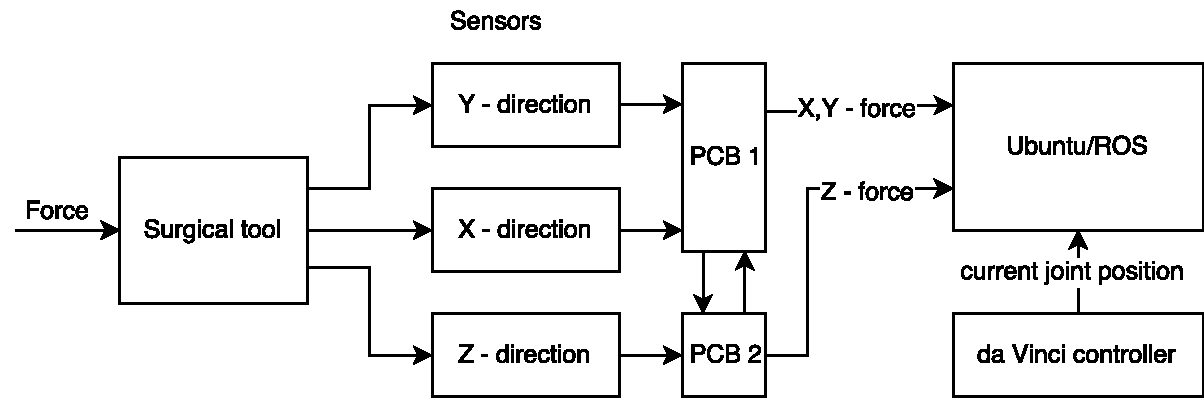
\includegraphics[width=140mm]{fig/methods/dbd2.pdf}
	\end{center}
	\vspace{-4mm}
	\caption[Block Diagram]
	{Block Diagram}
	\label{fig:BlockDiag}
	\vspace{-2mm}
\end{figure}

\section{Sensor Placement Optimization}
\label{sec:SimMod}
A finite element analysis was done in Solidworks to assess better placement of the strain gauges on the created device. In order to run finite element analysis material properties, such as elastic modulus, poisson`s ratio, and density are necessary to know. Sleeve material is aluminum 6061, that has elastic modulus 68.9 GPa, poisson`s ratio 0.33, and density 2700 kg/m\textsuperscript{3} \cite{aluminum_properties}. Since the shaft and cannula materials are unknown, in order to run finite element analysis their elasticity modulus and density were found experimentally.
	
	\subsection{Elastic Modulus Measurements}
	\label{sec:ElasMod}
	Elastic Modulus of the shaft and the cannula were found experimentally (Figure \ref{fig:ElasModSet}). One end of the observing sample (shaft/cannula) was fixed and the force was applied on the other end. We used weights 250g for the shaft and 555g for the cannula to apply forces. The deformation caused by forces was detected with dial indicator. Experiment was done 5 times, average displacement value was used to calculate elastic modulus. Results are shown in Table \ref{tab:elasMod}.
	
\begin{figure}[h]
	\begin{center}
		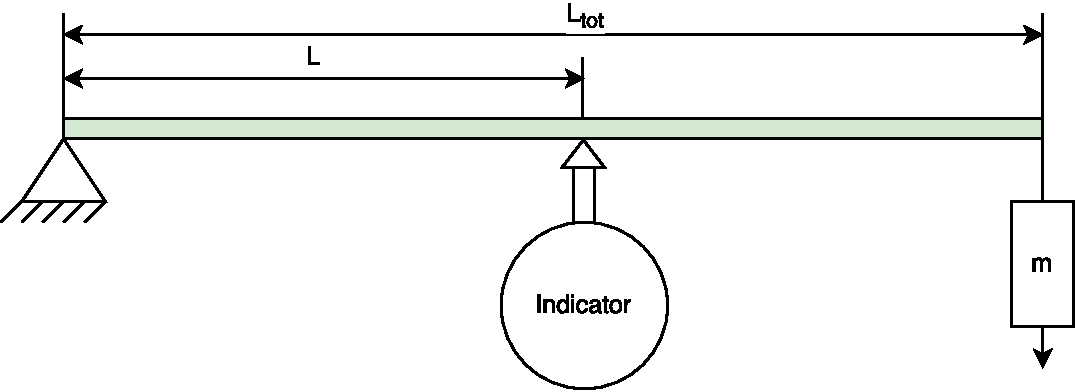
\includegraphics[width=120mm]{fig/methods/el_mod_set.pdf}
	\end{center}
	\vspace{-4mm}
	\caption[Setup to Measure Elastic Modulus]
	{Setup to Measure Elastic Modulus}
	\label{fig:ElasModSet}
	\vspace{-2mm}
\end{figure}

\begin{table}
\caption {Elasticity Modulus Measurement Data} \label{tab:elasMod} 
\begin{tabular}{ | c | c | c | c | c | c | c | c | } 
\hline
Component & $d_o$, mm & $d_i$, mm & $I$, mm\textsuperscript{4} & $m$, g & $F$, N & $L$, mm & $L_{tot}$, mm \\ 
\hline
Shaft & 8.4 & 6 & $1.808 \cdot 10^{-10}$ & 250 & 3.25 & 276.2 & 366.8\\ 
\hline
Cannula & 10.54 & 8.75 & $3.181 \cdot 10^{-10}$ & 555 & 6.011 & 95.5 & 105.55 \\ 
\hline
\end{tabular}

\begin{tabular}{ | c | c | c | } 
\hline
Component & $\delta \pm SD$, mm & $E \pm SD$, GPa \\ 
\hline
Shaft & $2.856 \pm 0.123$ & $44.31 \pm 1.86$ \\ 
\hline
Cannula & $0.086 \pm 0.004$ & $63.92 \pm 2.97$ \\ 
\hline
\end{tabular}
\end{table}

Elastic Modulus was found using following equation:

\begin{equation}
E = \frac{FL^3}{3 \delta I} 
\end{equation}

where $F$ - force, $L$ - length from the fixed point to indicator, $I$ - area moment of inertia, $\delta$ - displacement.

Area moment of Inertia: 
\begin{equation}
I = \frac{\pi (d_o^4 - d_i^4)}{64}
\end{equation}

where $d_o$ - cylinder outside diameter, $d_i$- cylinder inside diameter.

Force acting on indicator:
\begin{equation}
F = \frac{L_{tot}}{L}mg
\end{equation}

where $L_{tot}$ - total length of the object, $m$ - mass of the weight, $g$ - gravitational constant.

Experimentally found mean value of elastic modulus of the shaft is equal to 44.31 GPa with standard deviation (SD) 1.86 GPa, elastic modulus of the cannula is 63.92 GPa with SD 2.97 GPa.

	\subsection{Density Measurements}
	\label{sec:DenMeas}
Density was found using following equation:

\begin{equation}
p=\frac{m}{V}
\end{equation}

where $m$ - mass, $V$ - volume.

Weight was measured using mechanical scale. Volume of the shaft was found by following equation: $V =  \pi h(r_o^2-r_i^2) = 4.36 \cdot 10^{-5} m^3$. Volume of the cannula was found using water displacement method. Shaft material density is 473 kg/m\textsuperscript{3}, cannula material density is 55238 kg/m\textsuperscript{3}.

\subsection{Simulation Results}
\label{sec:FEAres}
The mounting location of the active strain gauges should be under the greatest amount of strain. From the Figure \ref{fig:XYdev}, it can be seen that strain gauges for X-Y direction device should be mounted on the area shown green, that corresponds to strain value approximately equal to $1.5 \cdot 10^{-4}$. Passive strain gauges, that will be used only for temperature compensation, will be placed on the blue area perpendicular to the active strain gauges.

\begin{figure}[h]
	\begin{center}
		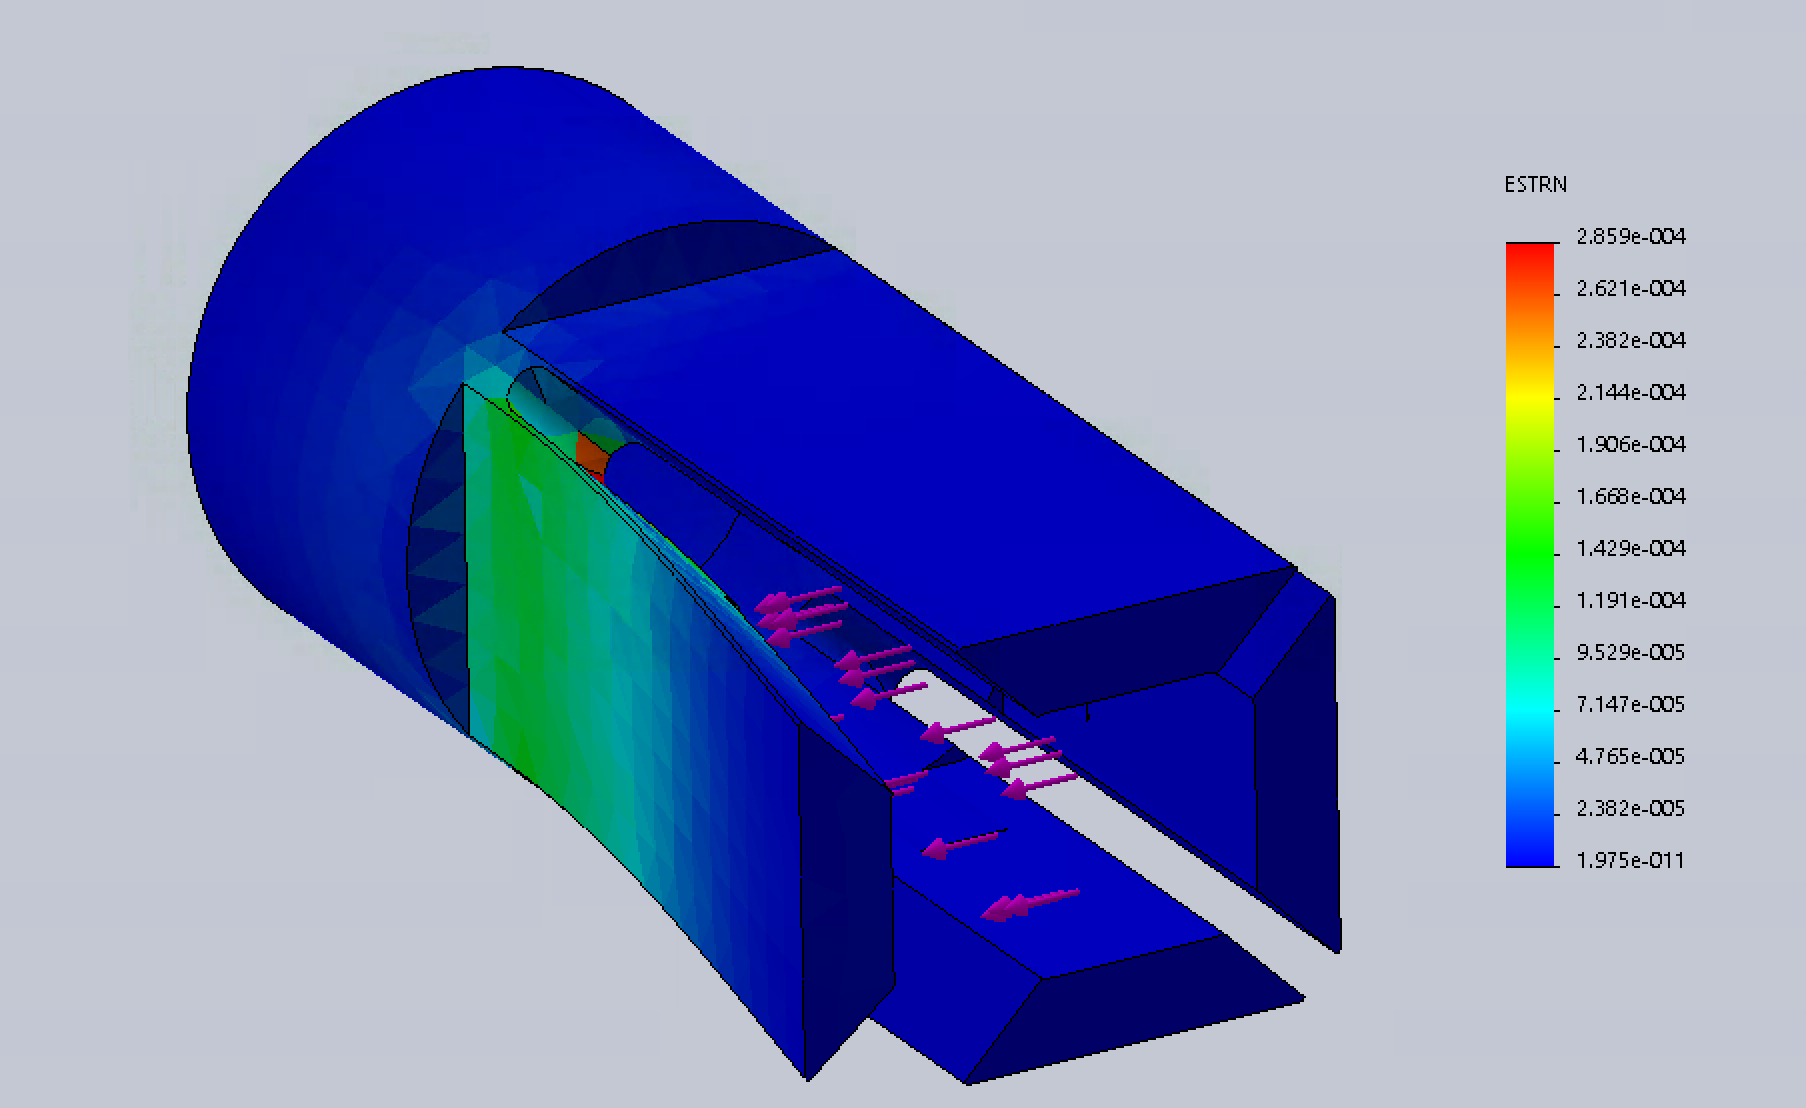
\includegraphics[width=100mm]{fig/methods/old_sleeve.png}
	\end{center}
	\vspace{-4mm}
	\caption[Strain in the Device to Measure Forces in X-Y Direction]
	{Strain in the Device to Measure Forces in X-Y Direction}
	\label{fig:XYdev}
	\vspace{-2mm}
\end{figure}


\begin{figure}[h]
	\begin{center}
		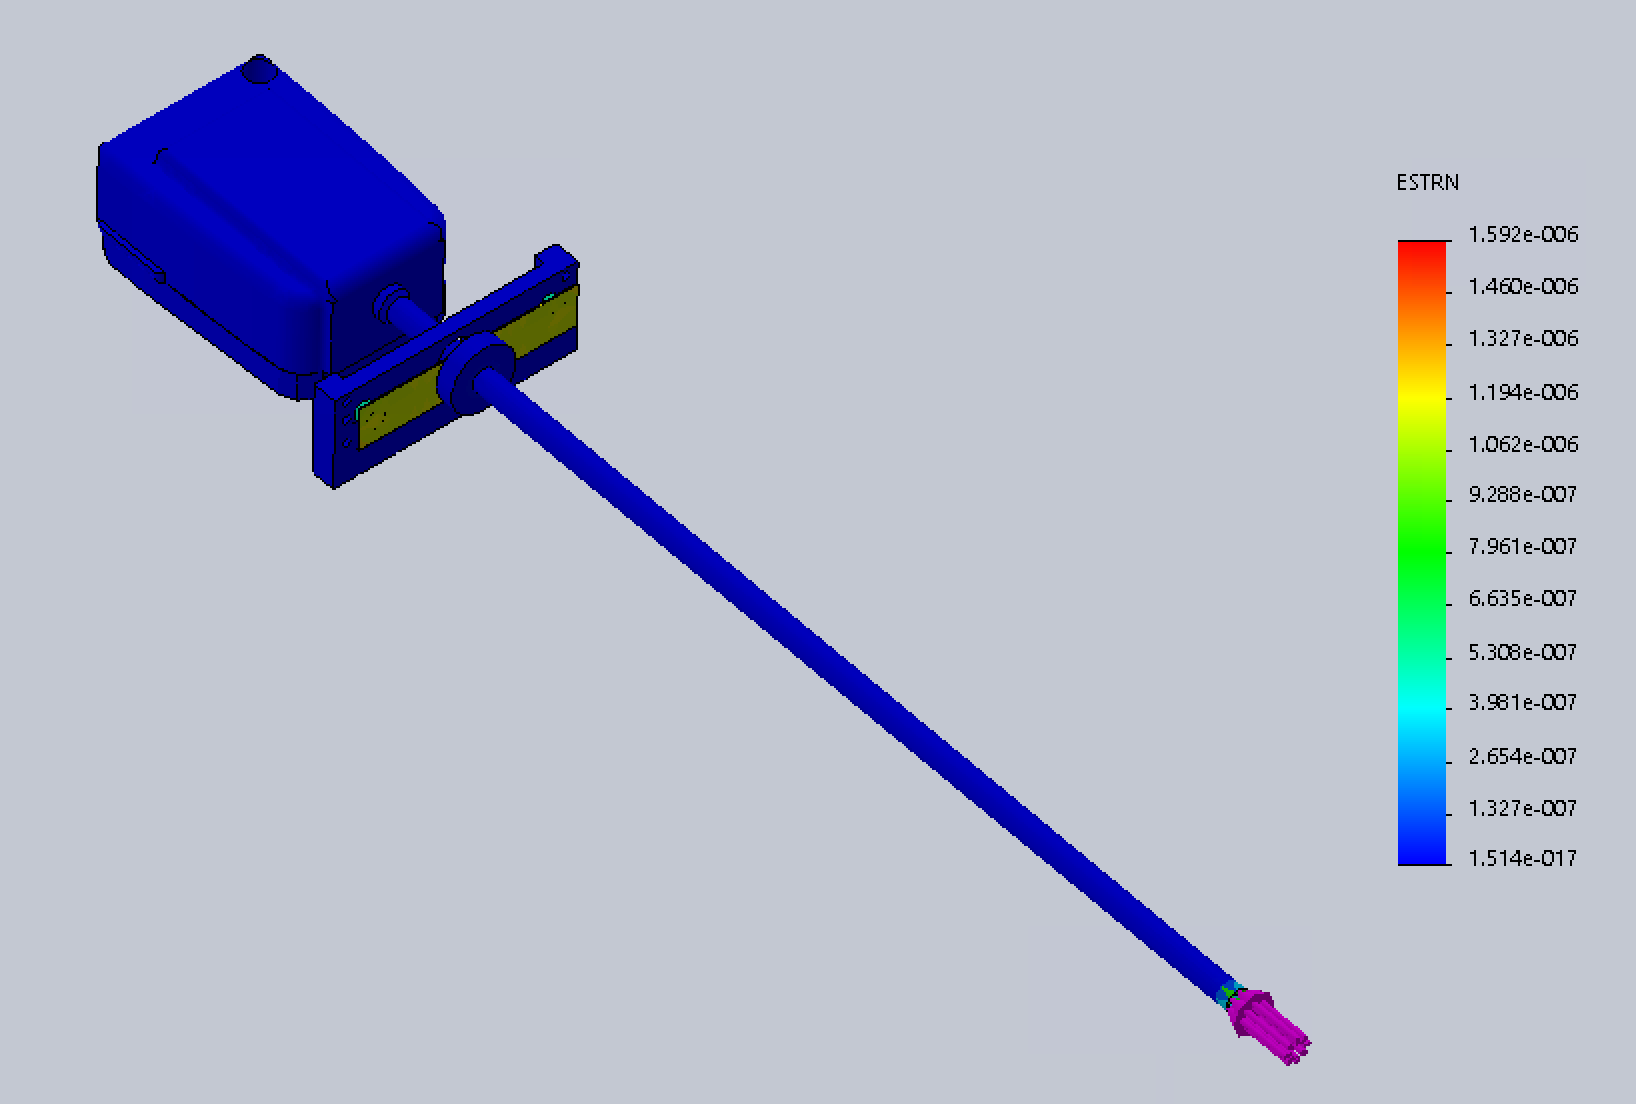
\includegraphics[width=100mm]{fig/methods/z_dir_sim.png}
	\end{center}
	\vspace{-4mm}
	\caption[Strain in the Device to Measure Forces in Z Direction]
	{Strain in the Device to Measure Forces in Z Direction}
	\label{fig:Zdev}
	\vspace{-2mm}
\end{figure}

For Z-direction measurement forces (Figure \ref{fig:Zdev}), area shown with yellow-green color under the highest strain. On both sides and both ends of this plate strain gauges should be placed to form full bridge.

\begin{table}
\caption {Material Properties} \label{tab:matProp} 
\begin{center}
\begin{tabular}{ | c | c | c | c | c | c | c | c | } 
\hline
Component & Elastic Modulus, GPa & Density, kg/ m\textsuperscript{3} \\ 
\hline
Shaft & 44.31 & 473\\ 
\hline
Cannula & 63.92 & 55238 \\ 
\hline
Sleeve & 68.9 & 2700  \\ 
\hline
\end{tabular}
\end{center}
\end{table}

All material properties used for simulations are listed in Table \ref{tab:matProp}.

\section{Requirements for the Device}
	\label{sec:DevReq}
	From the literature review, following requirements for the device were outlined:
	
	Biocompatibility: Z-device is attached to sterile adapter and does not have to be biocompatible. X-Y device goes inside the patient, it means that it should be sterilized and created using biocompatible materials. Current version of the device is not biocompatible. We can achieve biocompatibilty by using Stainless Steel as a device material and biocompatible epoxy to cover strain gauges, also teflon coated wires should be used for all electrical connections.
	
	Force range: Some studies \cite{mack_interactive_2012, prasad_modular_2003, } have shown that force range applied during surgeries lies in range (0-11 N). The designed device measures forces in that range, and if the force goes beyond that range it can be used to trigger safety alert.
	
	Force sensitivity: The device should be sensitive enough with minimum detectable signal (MDS) at least 0.3 N and give accurate readings (error < 0.05 N) \cite{mack_interactive_2012}.
	
	Speed of force reading: Device is used for real-time haptic feedback, the minimum requirement for data acquisition speed is 1 kHz \cite{seungmoon_choi_effect_2004}.
	
	No restriction of motion range of the device: We were able to measure force in three directions independently from each other using separate wheatstone bridges for each direction. At the same time tool can rotate freely and change depth of insertion.	
	
	Linearity: Strain gauges have linear response with deformation. Our calibration results have shown linearity of the readings.

	Device modularity: Force-sensing devices were designed to fit daVinci cannula and sterile adapter and compensate tolerances by adjustment of set screws.
	
\section{Mechanical Design}
\label{sec:mechDes}

	\subsection{Strain Gauge}
	\label{sec:SGReq}
	According to the manual for strain gauge selection provided by Vishay Micro-Measurements, the strain gauge should have following parameters:
\begin{itemize}
  \item Single grid for unidirectional force measurements;
  \item Isoelastic (D alloy) that has higher gauge factor with E backing;
  \item Encapsulated with pre attached leads for easier placement;
  \item STC (self-temperature-compensation) - small temperature dependence;
\end{itemize}	
	
Maximum strain on the created device is $1.5 \cdot 10^{-4}$, in case of 10 N load with maximally opened shaft. From the literature, strain gauges length should be more than 5\% of maximum strain, hence, minimum length of the strain gauge should be 0.0075 mm. 

Gauge Factor (GF) for strain gauges usually is 2. According to the formula (\ref{eq:resistance}) strain gauge with resistance 120 $\Omega$ have maximum change in resistance equal to 0.036 $\Omega$, and 350  - 0.105 $\Omega$:

\begin{equation}\label{eq:resistance}
\Delta R=GF \cdot R \cdot \varepsilon
\end{equation}

where $GF$ - gauge factor, $R$ - resistance, $\varepsilon$- strain.

For the device strain gauges with resistance 350 $\Omega$, GF is 2, single grid, encapsulated with pre-attached leads were used.

	\subsection{Installation of Strain Gauges}
	\label{sec:instSG}

	Application of strain gauges was done following the manual provided by Vishay Micro-Measurements. \cite{StrGugeInst}.

	First the working surface (glass) and tweezers were cleaned with Neutralizer 5. 
	After that shaft surface preparation was started, using solvent degreaser GC-6 Isopropyl Alcohol. 
	A gauge layout was then applied with a 4H drafting pencil. The surface was then conditioned with Conditioner A and the extra liquid was wiped with gauze. 
	Finally, the surface was then neutralized with M-Prep Neutralizer 5A. \cite{StrGugeInst}

	The strain gauges were first placed on the glass and then transported using mylar tape onto the instrument surface. A thin layer of catalyst was applied on the strain gauge and given one minute to dry. Then adhesive M-BOND 200 was applied on the surface, pressure was applied on the tape for one minute, then two more minutes to let it dry before the tape was removed. Then leads soldering was done by application of pats, and soldering them with thin wires. \cite{youtube}

	The methodology of the strain gauge application more specifically described in \cite{StrGugeInst}.

	In compliance with the literature \cite{StrGugeInst} for application of the strain gauge on metals, the same materials and technique can be used. Therefore, the same method was used to apply strain gauges on different materials.

\subsection{X-Y Device}
\label{sec:xyDir}

XY-device consists of one sleeve and one set screw. We manufactured sleeve using Aluminum 6061 Alloy. %First, hole with diameter 9.5 mm should be drilled in the center using the lathe machine. Then on the milling machine all the side slots and inner square should be milled. On the same machine hole for the set screw should be drilled. After that set screw thread was tapped.%
The manufactured sleeve is placed on the cannula end and is fixed with a set screw on the top.

\begin{figure}[h]
	\begin{center}
		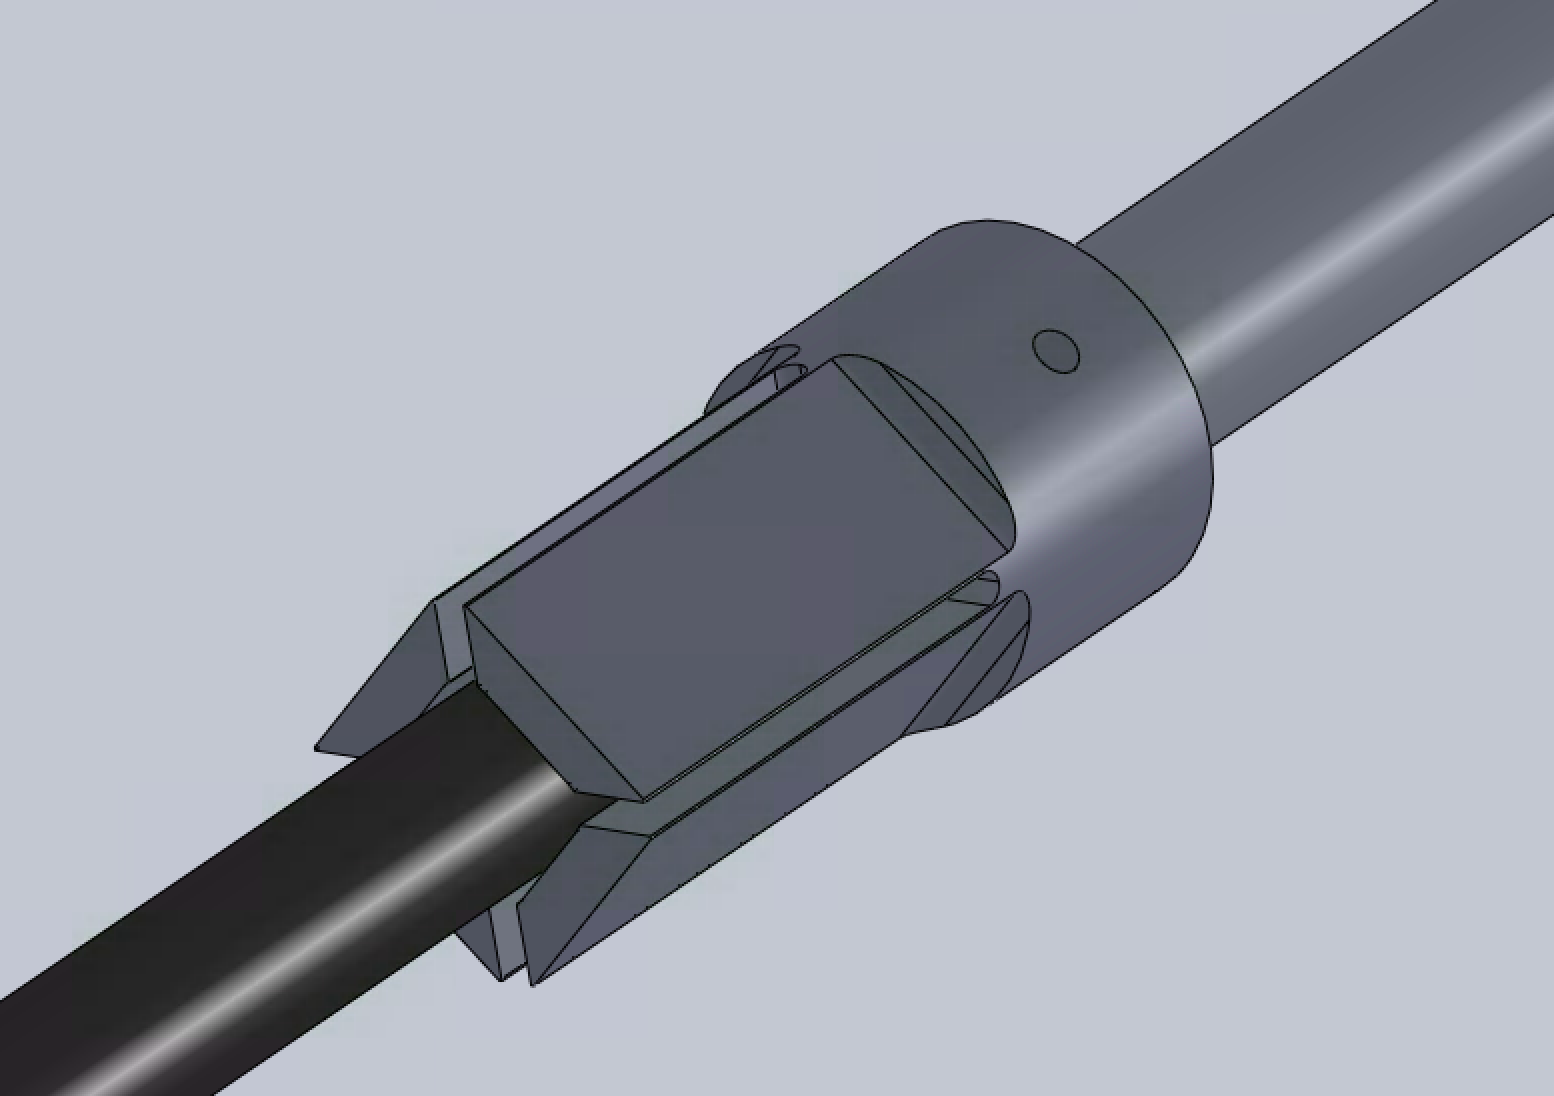
\includegraphics[width=80mm]{fig/methods/xy_dev_cl.png}
	\end{center}
	\vspace{-4mm}
	\caption[XY-direction Force Feedback Sensor]
	{XY-direction Force Feedback Sensor}
	\label{fig:xy-direction}
	\vspace{-2mm}
\end{figure}

\begin{figure}[h]
	\begin{center}
		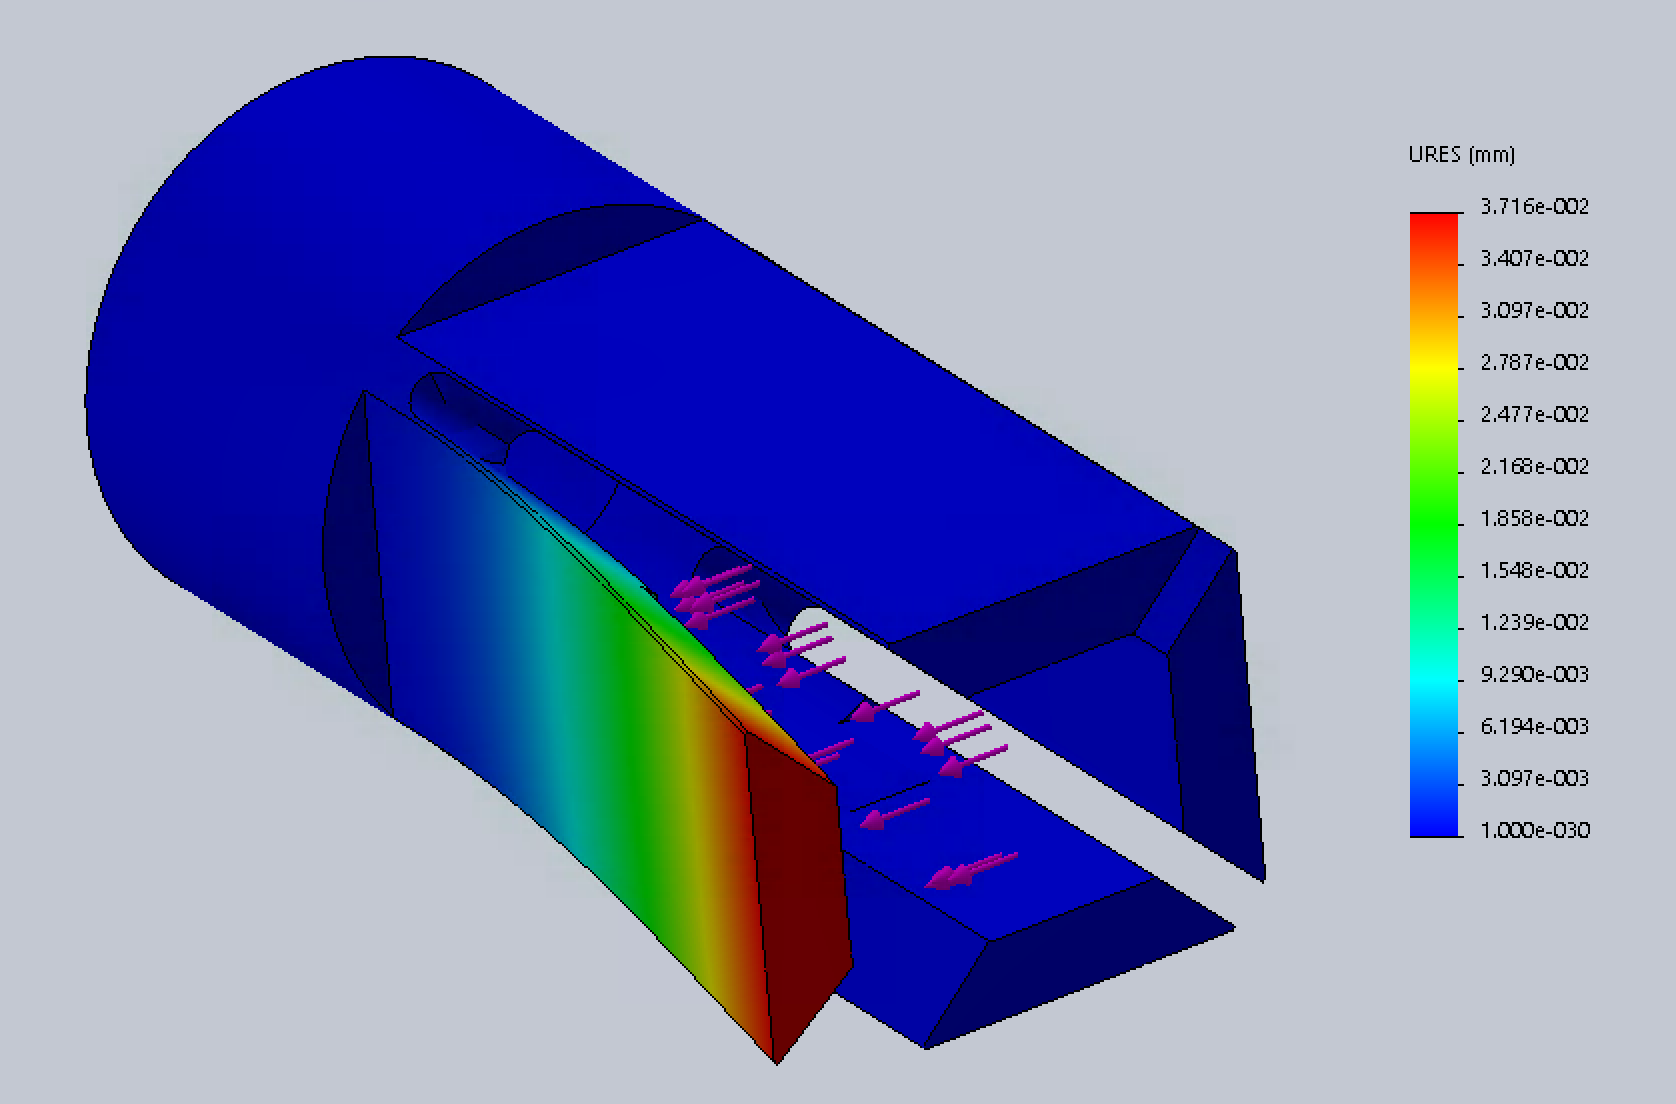
\includegraphics[width=80mm]{fig/methods/old_sleeve_displ.png}
	\end{center}
	\vspace{-4mm}
	\caption[Displacement of the XY Device]
	{Displacement of the XY Device}
	\label{fig:xy-displ}
	\vspace{-2mm}
\end{figure}

In order to get accurate readings maximum displacement of the sleeve sides should prevent shaft from hitting the cannula. It means that it should be less than $d=(d_{can_in} - d_{shaft_out})/2 = (8.75 - 8.4)/2 = 0.175$ mm. From the Solidworks simulation (Figure \ref{fig:xy-displ}), maximum displacement is 0.037 mm, which is in appropriate range.

\subsection{Z Device}
\label{sec:zDir}

\begin{figure}[h]
	\begin{center}
		\includegraphics[width=80mm]{fig/methods/z_dir_design.png}
	\end{center}
	\vspace{-4mm}
	\caption[Z-direction Force Feedback Sensor]
	{Z-direction Force Feedback Sensor}
	\label{fig:Z-direction}
	\vspace{-2mm}
\end{figure}

\begin{figure}[h]
	\begin{center}
		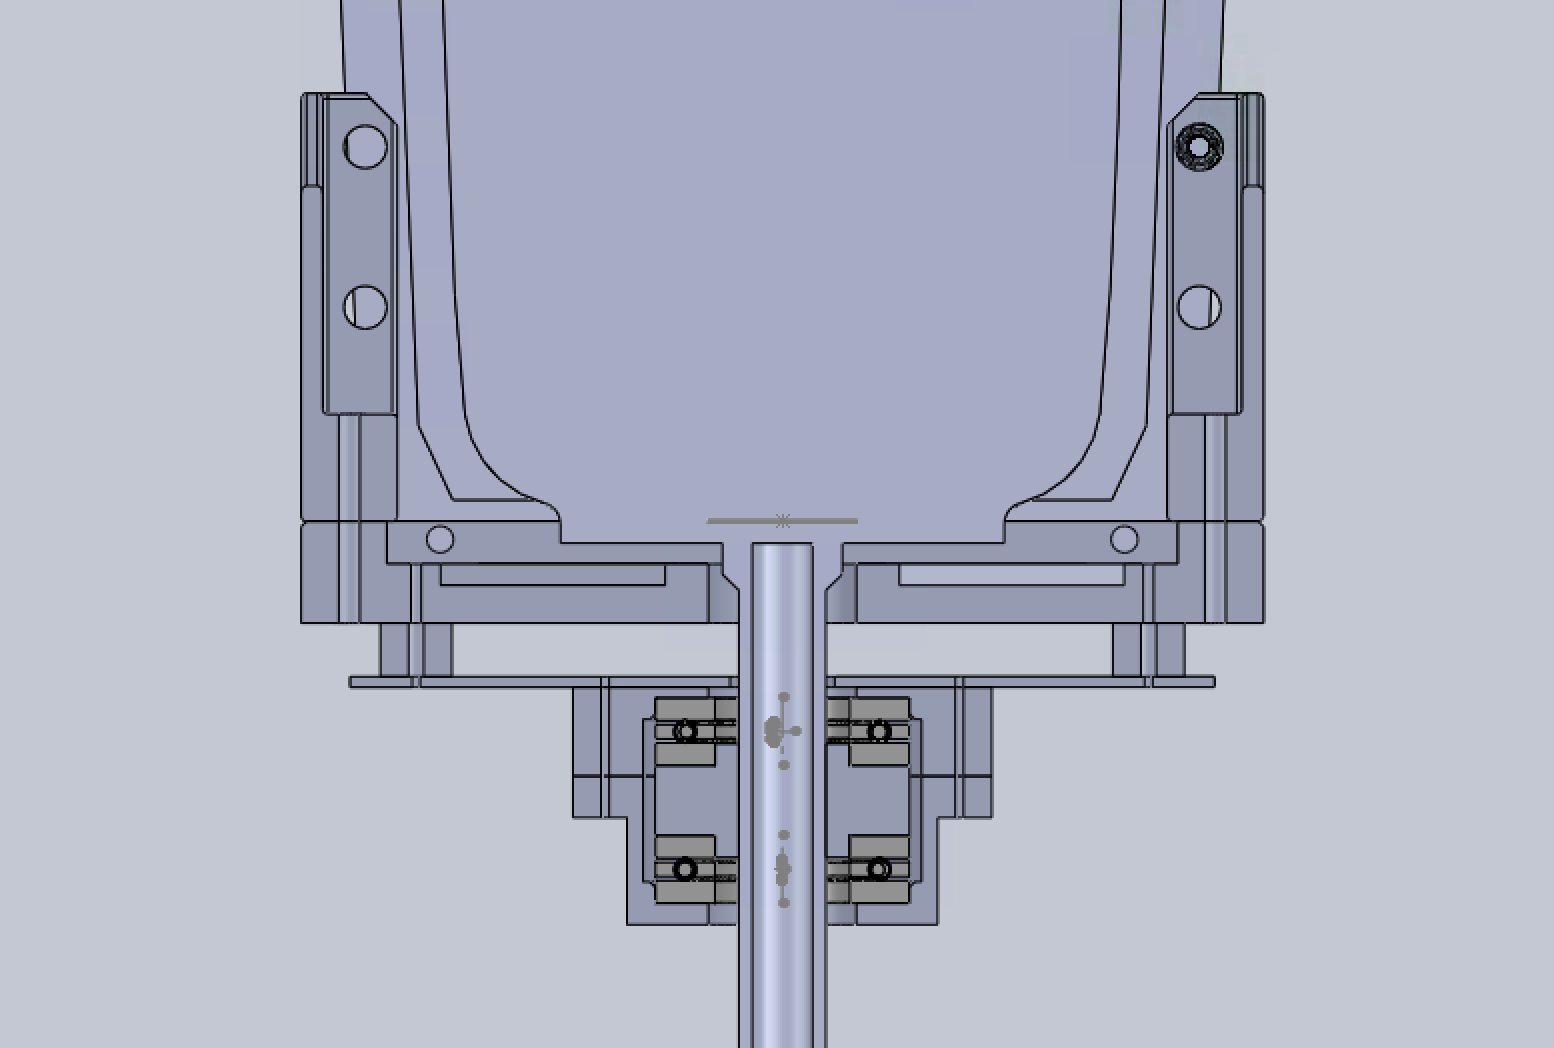
\includegraphics[width=80mm]{fig/methods/z_dir_sec.png}
	\end{center}
	\vspace{-4mm}
	\caption[Z-direction Force Feedback Sensor (Section View)]
	{Z-direction Force Feedback Sensor (Section View)}
	\label{fig:Z-direction_sec}
	\vspace{-2mm}
\end{figure}


Z-device (Figures \ref{fig:Z-direction}, \ref{fig:Z-direction_sec}) consists of attachment to the sterile adapter, 2 thrust ball bearings, three rings, plate, and two cylindrical spacers. Three rings and two ball bearings are used to transfer only z-directional forces further to the plate and keep ability of the shaft to rotate. The ring in the center is in direct contact with the instrument shaft, two outer rings are for the push and pull forces transfer. The plate experience maximum strain and all strain gauge sensors are mounted on it.  Two cylindrical spacers are used to give plate space to move and they are mounted on the attachment plate. the attachment plate consist of three plates, they are press fitted on the sterile adapter and fixed with four set screws.

Three rings and plate were manufactured with Aluminum Alloy 6061, attachment parts were 3-D printed, fasteners were used as spacers.


\section{Electrical and Software Design}
\label{sec:elecDes}

	\subsection{Circuit design}
	\label{sec:cirDes}
	Block diagram of the developed PCB is shown on Figure \ref{fig:PCB_block_diag}. Signal waveforms are shown on Figure \ref{fig:Wave_Out}.

\begin{figure}[h]
	\begin{center}
		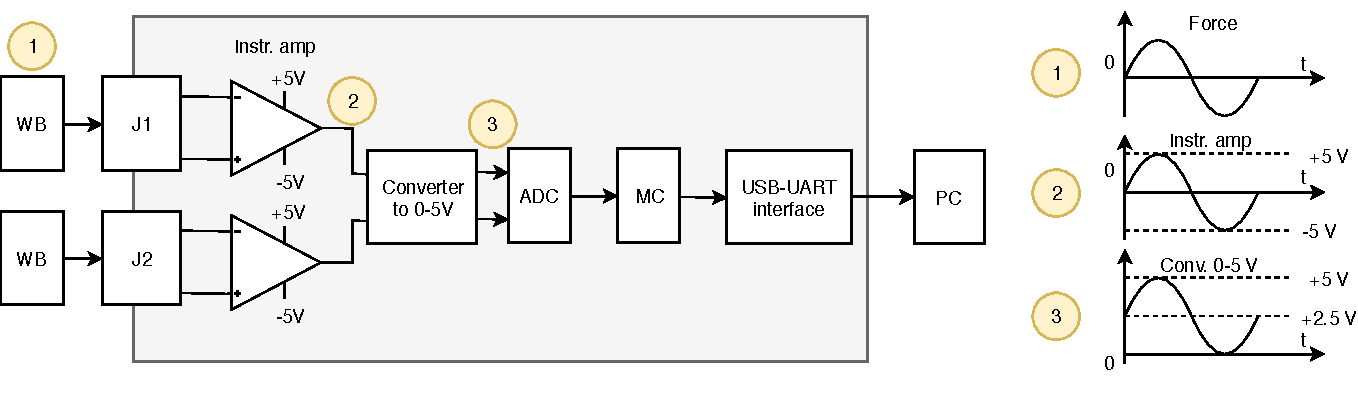
\includegraphics[width=150mm]{fig/methods/PSC_block_wave.pdf}
	\end{center}
	\vspace{-4mm}
	\caption[Block Diagram of the Circuit]
	{Block Diagram of the Circuit}
	\label{fig:PCB_block_diag}
	\vspace{-2mm}
\end{figure}
%\begin{figure}[h]
%	\begin{center}
%		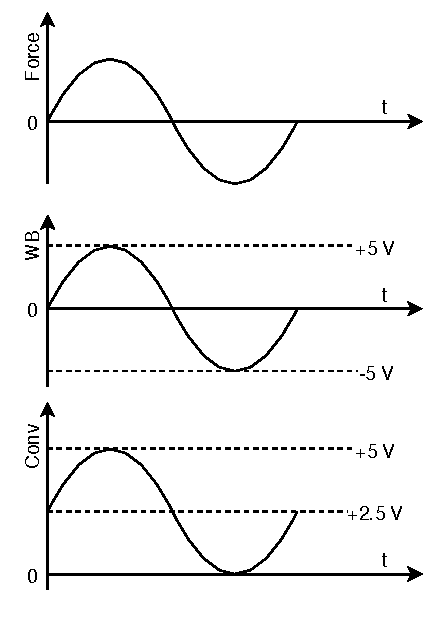
\includegraphics[width=60mm]{fig/methods/signal_diag.pdf}
%	\end{center}
%	\vspace{-4mm}
%	\caption[Signal Waveforms]
%	{Signal Waveforms}
%	\label{fig:Wave_Out}
%	\vspace{-2mm}
%\end{figure}

Four strain gauges are connected to form a wheatstone bridge circuit. On Figures \ref{fig:WB_xy_dev} - \ref{fig:WB_z} placement of strain gauges (1-4) and their wheatstone bridge configurations are shown for both devices. Strain gauges deform due to applied forces, and it causes voltage change on wheatstone bridge. Output signal from the wheatstone bridge goes to the instrumentation amplifier. Since ADC can convert only positive voltage, voltage converter changes voltage range of the output signal from ($-5V$ to $+5V$) to ($0V$ to $+5V$) range. That signal is converted to digital signal with 16-bit ADC, which communicates with the microcontroller via SPI interface. The output signal is transferred to the computer via USB. 
	
\begin{figure}[h]
	\begin{center}
		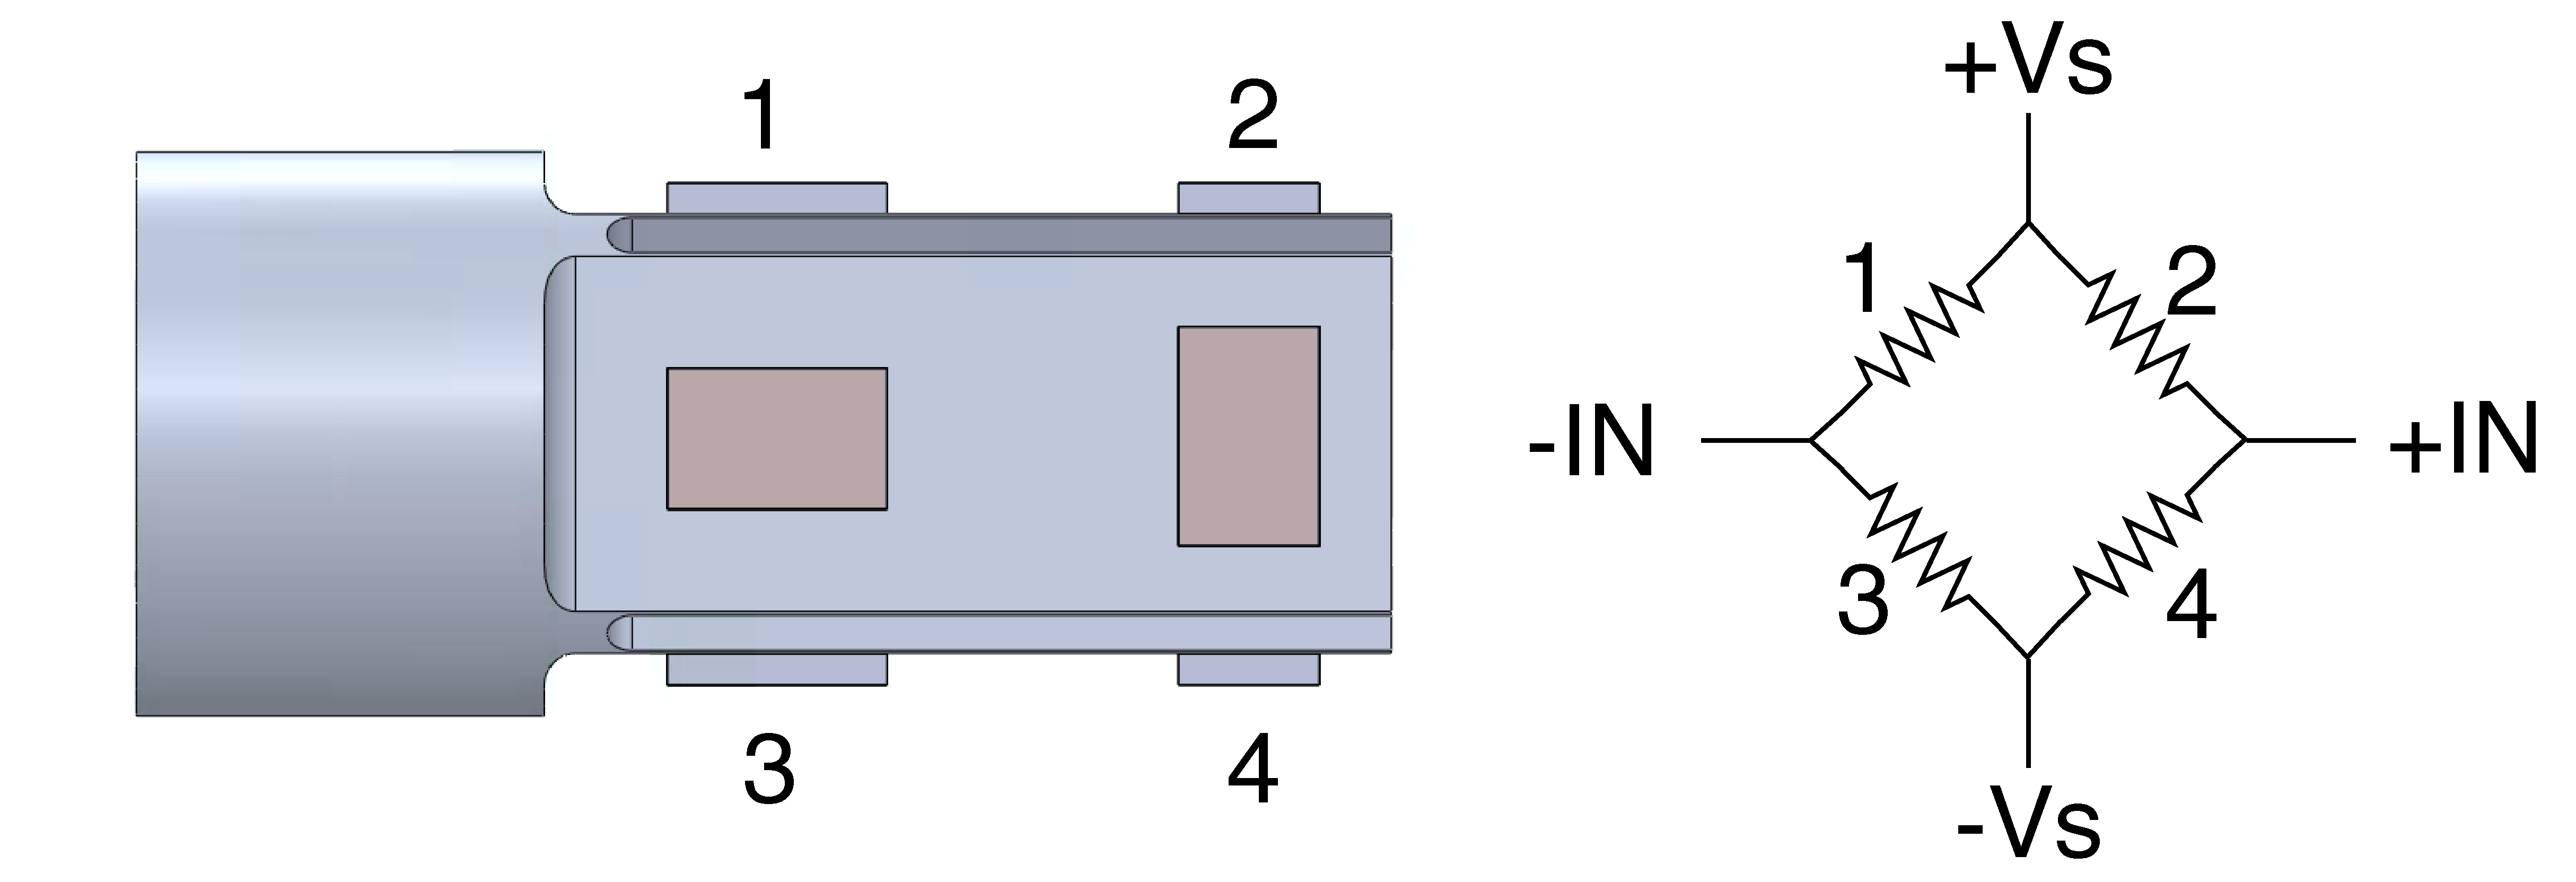
\includegraphics[width=120mm]{fig/methods/Wiring_xy_sleeve.pdf}
	\end{center}
	\vspace{-4mm}
	\caption[Wheatstone Bridge Configuration of the XY-device]
	{Wheatstone Bridge Configuration of the XY-device}
	\label{fig:WB_xy_dev}
	\vspace{-2mm}
\end{figure}

\begin{figure}[h]
	\begin{center}
		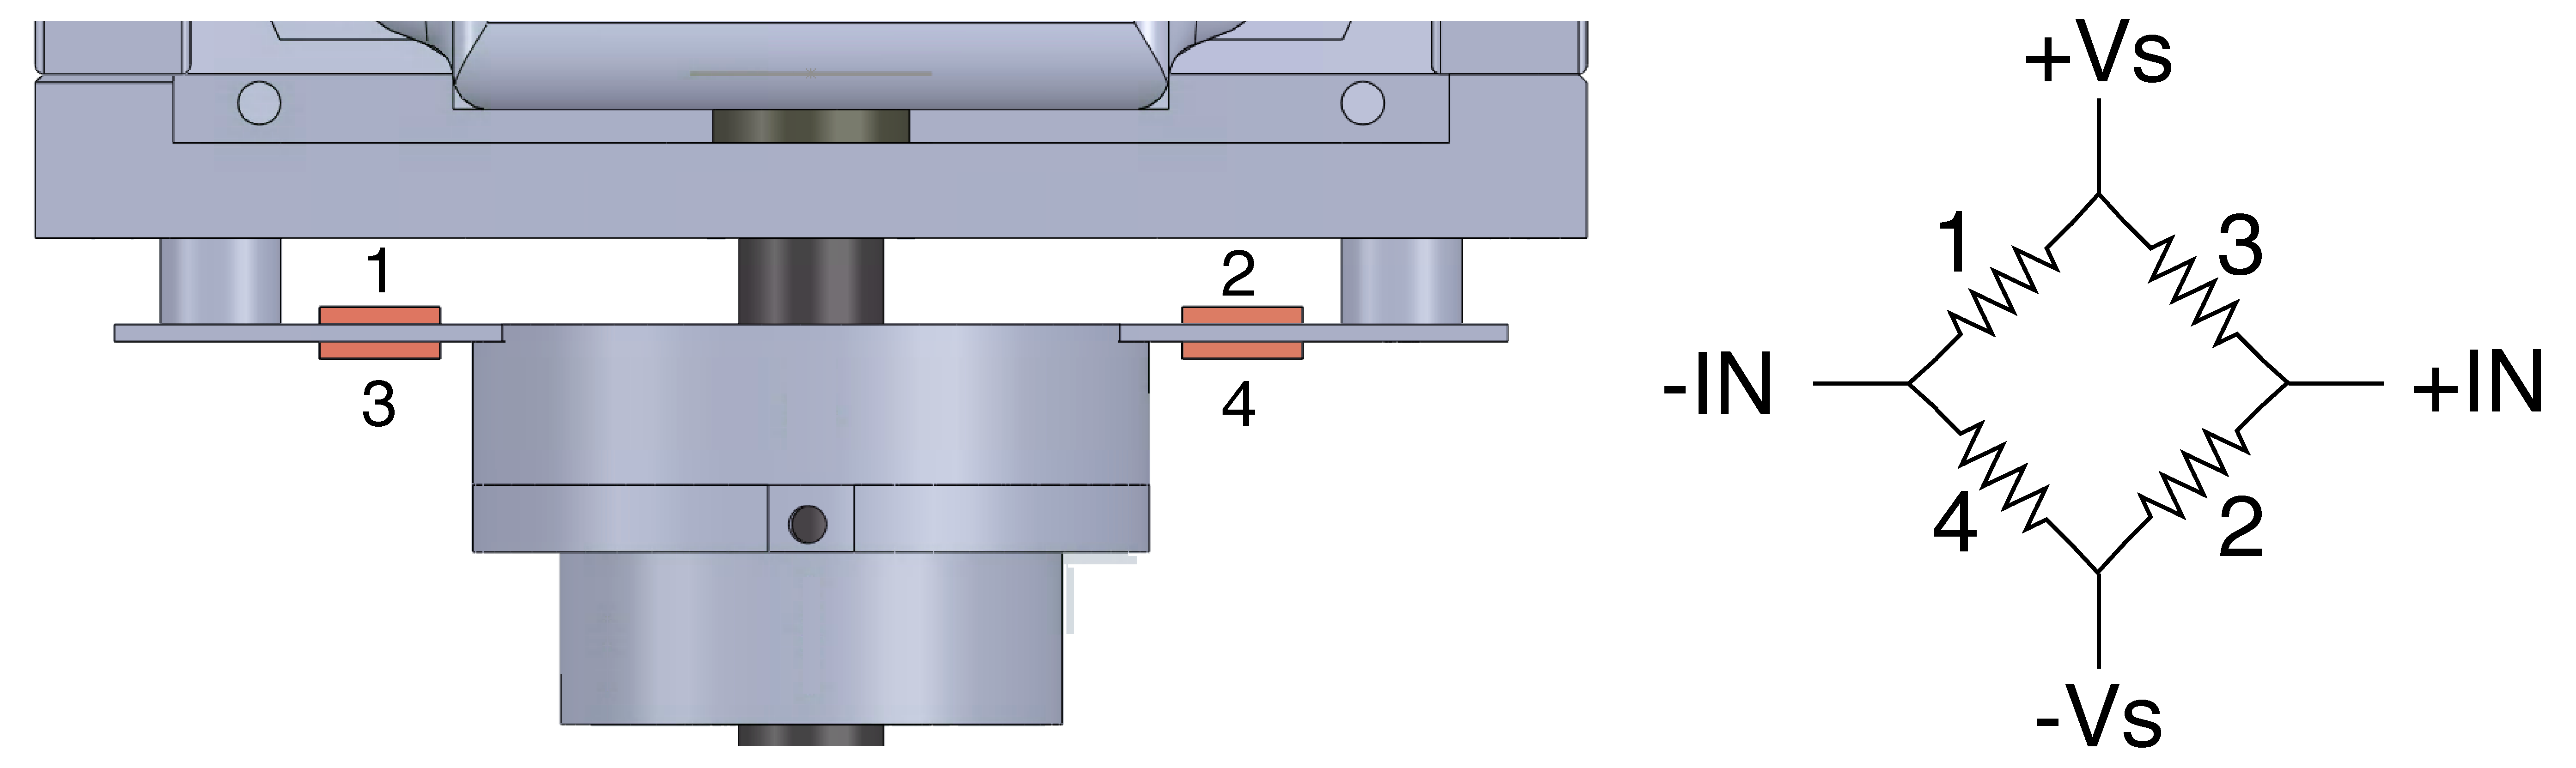
\includegraphics[width=140mm]{fig/methods/Wiring_z.pdf}
	\end{center}
	\vspace{-4mm}
	\caption[Wheatstone Bridge Configuration of the Z-device]
	{Wheatstone Bridge Configuration of the Z-device}
	\label{fig:WB_z}
	\vspace{-2mm}
\end{figure}
	
\begin{figure}[h]
	\begin{center}
		\includegraphics[width=120mm]{fig/methods/PCB_real_look.png}
	\end{center}
	\vspace{-4mm}
	\caption[Manufactured PCB]
	{Manufactured PCB}
	\label{fig:PCB_real}
	\vspace{-2mm}
\end{figure}
	
Using Altium Designer 15.1 the PCB design was developed and manufactured at Advanced Circuits \cite{PCB_manufacturer}. 

In the developed PCB (Figure \ref{fig:PCB_real}) trimpots are used for calibration of the instrumentation amplifier gain (shown yellow) and change of reference voltage (shown red).

Instrumentation amplifier gain change is needed to set up appropriate measuring force range (0-11 N). During calibration, when 11 N applied on the tool end, the output signal (that goes to ADC) should be smaller than 4 V. When the same force applied in the opposite direction, the output signal should be bigger than 1 V.
 
Reference voltage change is used for the compensation of wheatstone bridge unbalance caused by strain gauge resistance tolerances. During the calibration, it should be tuned until it gives the output signal close to 2.5 V, when no forces applied on the device.

More details on the developed PCB are on github link.

	\subsection{Noise Analysis}
	\label{sec:NoiseExp}
	Fast Fourier transform (FFT) waveform analysis of the noise signal was performed using Tektronix MSO 4034 Mixed Signal Oscilloscope. The oscilloscope automatically applied the Hanning window, which has good frequency resolution and reduced spectral leakage\cite{harris_use_1978}.
	
\begin{figure}[h]%
\centering
\subfigure[1st Channel]{%
\label{fig:first}%
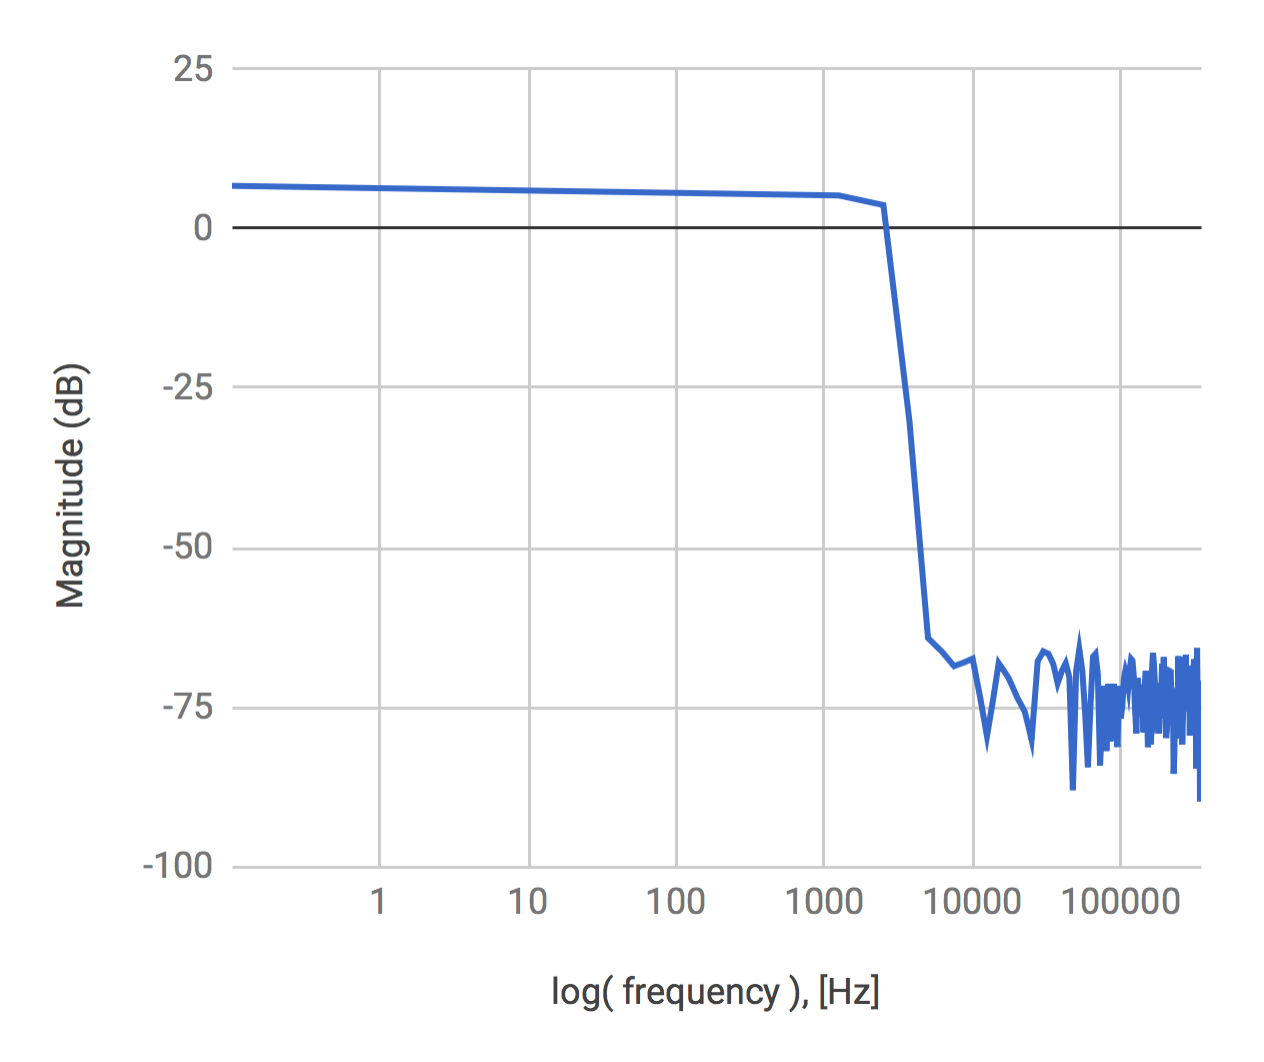
\includegraphics[height=2.2in]{fig/methods/noise_1_log.png}}%
\qquad
\subfigure[2nd Channel]{%
\label{fig:second}%
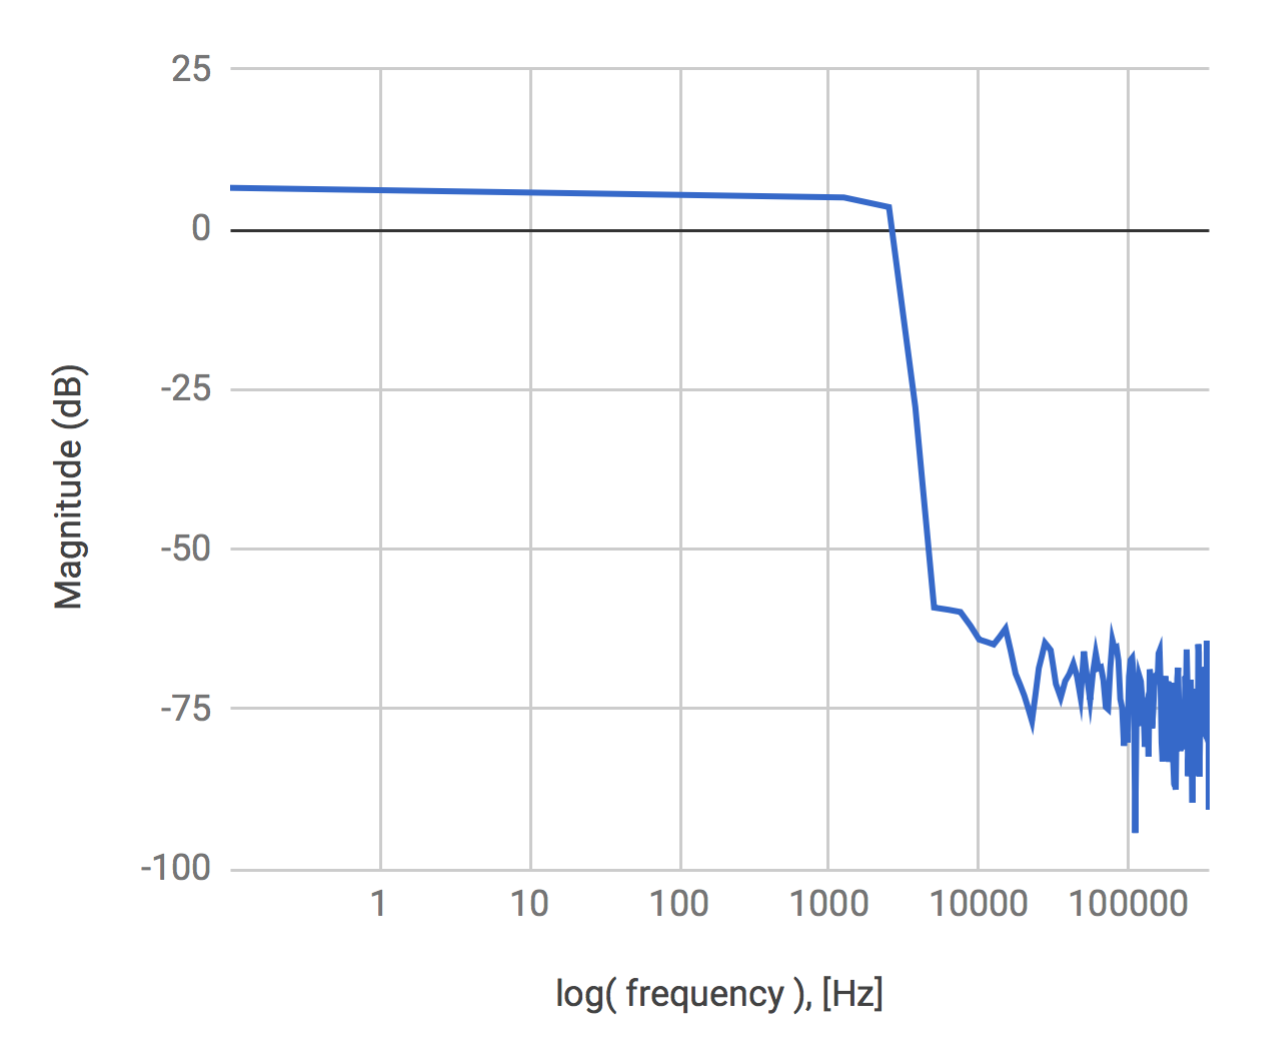
\includegraphics[height=2.2in]{fig/methods/noise_2_log.png}}%
\caption{FFT Analysis Results}
\end{figure}
	
	The signal frequency from the force sensor should be in range of (0 to 1 kHz). From the FFT analysis it can be concluded, that the noise frequency is in range (2.5 kHz and higher) with amplitude (-50 mV to 70 mV) for both channels. That means, low pass filter with cutoff frequency 2 kHz should be applied on the output signal. It was decided to use data averaging due to its simplicity of implementation and small time delays. It is an equivalent of low pass filtering that compensates the high frequency noise \cite{filtering_mov_ave}.

	\subsection{Microcontroller Software}
	\label{sec:MicrSoft}
	Microcontroller ATMEGA328P is used in the developed PCB for acqusition, filtering, and sending data to ROS. Main advantage of this microcontroller is that it has open-source packages for serial communication with ROS. The microcontroller is programmed to initialize ros nodes with names "adc\textunderscore xy" for XY-device and "adc\textunderscore zlc" for Z-device. The master-slave communication is created between X-Y and Z- devices for data acquizition synchronization by sending start conversion signals between two PCBs. When one of the devices gets the signal it starts to communicate with ADC though SPI interface (Figure \ref{fig:SPI_com}) \cite{introduction_SPI}. The acquired data is filtered from the high frequency noise by averaging of the 5 most recent readings. And the filtered data is published through the serial port with the baud rate 115200 bits per second. 
	
\begin{figure}[h]
	\begin{center}
		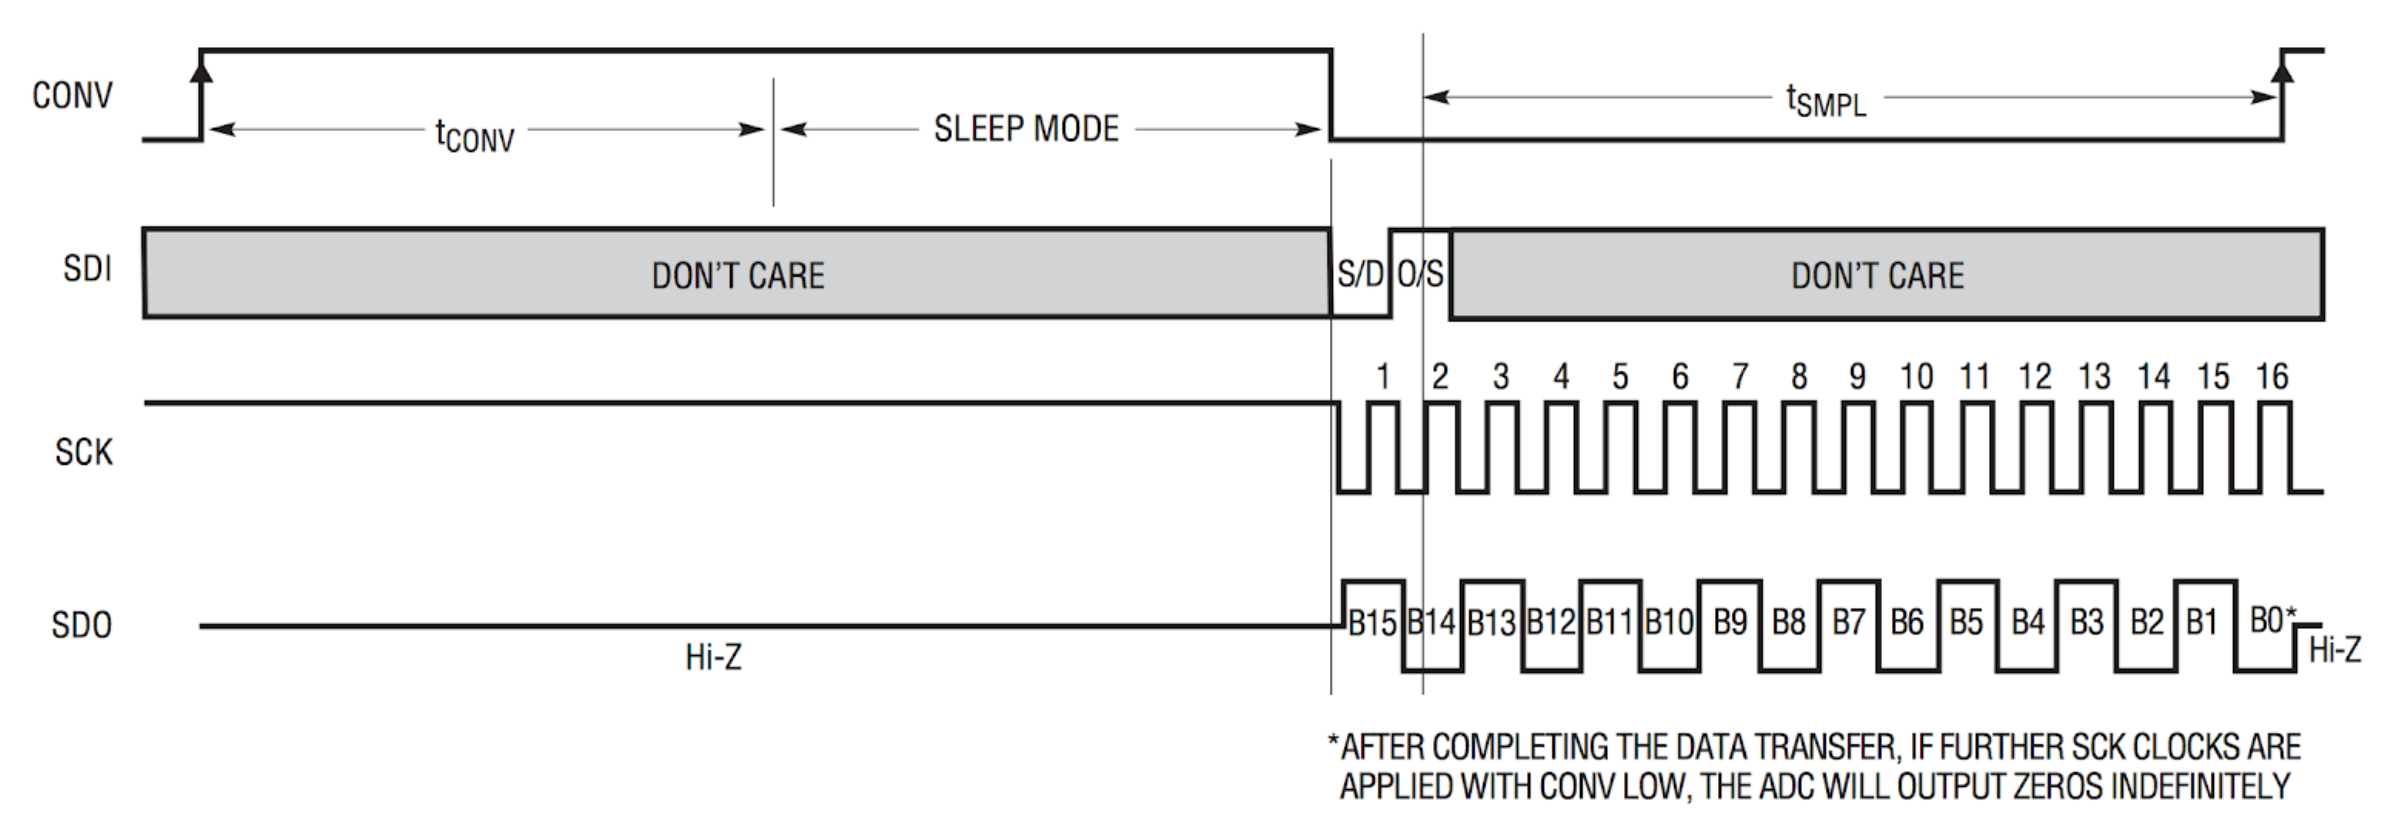
\includegraphics[width=140mm]{fig/methods/SPI_communication.png}
	\end{center}
	\vspace{-4mm}
	\caption[ADC LTC1865 Operating Sequence]
	{LTC1865 Operating Sequence \cite{ltc1865}}
	\label{fig:SPI_com}
	\vspace{-2mm}
\end{figure}

The github link to master device code and slave-device code.

	\subsection{ROS Architecture}
	\label{sec:p2}
Figure \ref{fig:ROS_arch} shows the ROS architecture of the developed system. In the python script we create a \textit{force\textunderscore feedback} node. The node is subscribed to X, Y, Z ADC data acquired form sensors and position of the sterile adapter from the daVinci controller. These data are used to find forces. The calculated forces (\textit{force\textunderscore x, force\textunderscore y, force\textunderscore z}) are then published.
\begin{figure}[h]
	\begin{center}
		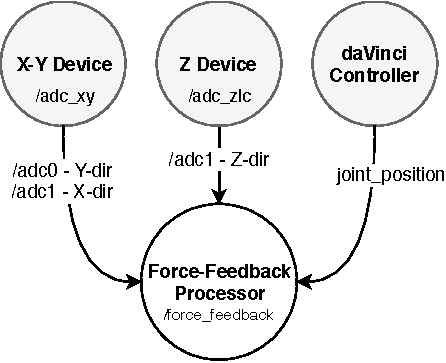
\includegraphics[width=80mm]{fig/methods/ROS_architecture.pdf}
	\end{center}
	\vspace{-4mm}
	\caption[ROS Architecture]
	{ROS Architecture}
	\label{fig:ROS_arch}
	\vspace{-2mm}
\end{figure}	

The program calculates magnitude of the forces in X, Y, Z directions using the calibration equation:
\begin{equation}\label{eq:calib_eq}
F = \frac{adc_{data} - b}{a}
\end{equation}

where $b$ is the constant equal to ADC reading when $F = 0$, $adc_{data}$ is current sensor reading in corresponding direction, and $a$ is linear function of sterile adapter position:
\begin{equation}\label{eq:ster_adap_pos}
a = c \cdot position + d
\end{equation}

where $c$ and $d$ are constants found during calibration and $position$ is the position of the sterile adapter.

Z-device readings does not depend on the position of the sterile adapter. Hence, $a$ has a constant value for Z-device.
 
	%To make communication between microcontroller and ROS work it is necessary to install rosserial\textunderscore arduino package \cite{rosserial_arduino}.
	
\section{Calibration}
\label{section:Calibration}

	\subsection{Calibration Setup}
	\label{sec:CalSetup}
	In order to find parameters of the calibration equation (\ref{eq:calib_eq}), the calibration system was developed (Figure \ref{fig:Calib_setup_BD}). The load cell and Polaris optical tracking system are used to find "true" force applied to the tool end. The load cell is used to find the magnitude of the applied force and the optical markers (4-5) to find the direction of the force.
	
	The calibration of the device starts with calibration of the load cell. The daVinci tool is inserted in the sterile adapter.  The force readings depend on the position of the sterile adapter, meaning that the force/sensor readings curve should be found for different positions of the adapter. Finding the curve for only two positions would be enough, because the correlation between the curve and position is linear, as the equation (\ref{eq:ster_adap_pos}) shows. 
	
\begin{figure}[h]
	\begin{center}
	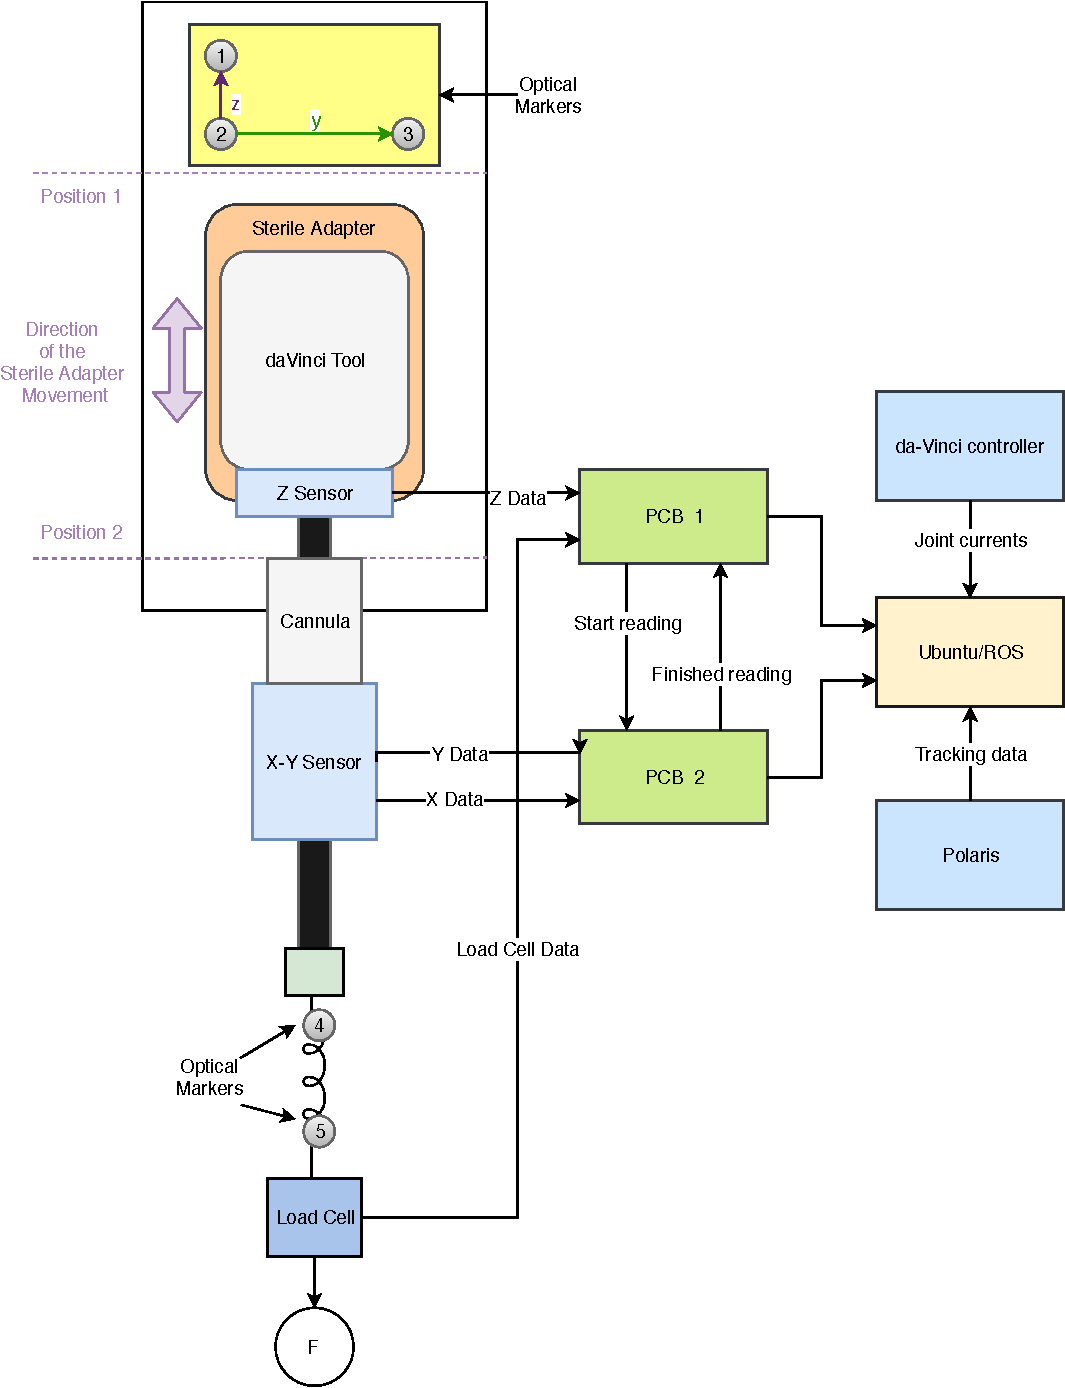
\includegraphics[width=105mm]{fig/methods/block_diagram_of_calib_setup.pdf}
	\end{center}
	\vspace{-4mm}
	\caption[Block Diagram of the Calibration Setup]
	{Block Diagram of the Calibration Setup}
	\label{fig:Calib_setup_BD}
	\vspace{-2mm}
\end{figure}

	Before starting a data collection, the PSM joint of the sterile adapter is fixed in the position 1. After fixing the adapter, in order to transform Polaris camera frame to the robot frame, the transformation matrix should be found. For this purpose, three optical markers (1-3) are attached to the PSM. Z-direction vector corresponds to the vector formed by optical markers (2-1), Y-direction vector is formed by optical markers (2-3). X-direction vector can be found as a cross product between these two vectors:
\begin{equation}
\vec{X} = \vec{Y}\times \vec{Z}
\end{equation}

	The transformation matrix $T_{c}^{ r}$ is found using coordinates of the $\vec{X}$, $\vec{Y}$, $\vec{Z}$ vectors and coordinates of the optical marker (2) defined as an origin vector.
\begin{equation}
T_{c}^{ r} = 
\begin{bmatrix}
    X_{x} 	& Y_{x} 		& Z_{x} 		&  x_{0} \\
    X_{y} 	& Y_{y} 		& Z_{y} 		&  y_{0} \\
    X_{z} 	& Y_{z} 		& Z_{z} 		&  z_{0} \\
    0		 	& 0 			& 0 			& 1
\end{bmatrix}
\end{equation}

	After finding the transformation matrix, the data collection starts. Polaris publishes coordinates of the optical markers (4-5). These coordinates are transformed to the robot frame:
\begin{equation}
P_{r} = {T_{c}^{ r}}^{-1} \cdot P_{c}
\end{equation}

	where $P_{r}$ - coordinates of the marker in the robot frame, $P_{c}$ - coordinates in the camera frame.
	
	The unit vector of the applied force is found in the robot frame:
\begin{equation}
\vec{U} = \frac{P_{5} - P_{4}}{|P_{5} - P_{4}|}
\end{equation}
	
	where $P_{5}$ is the position of the optical marker (5), $P_{4}$ is the position of the marker (4), they both are in the robot frame.
	
	The vector of the applied force in the robot frame can be found:
\begin{equation}
\vec{F} = F_{m} \cdot \vec{U}
\end{equation}

	where $F_{m}$ is the force magnitude found using the load cell.
	At the same time data from X, Y, Z sensors is collected. The collected data is used to find calibration equation parameters.
	
	\subsection{Calibration of the Load Cell}
	\label{sec:CalLoadCell}
	The calibration of the load cell is a part of the calibration process of the created device. The bloack diagram of the setup for the load cell calibration is shown on Figure \ref{fig:Calib_setup_LC}. The force $F$ was applied on the load cell using weights, its value: 
\begin{equation}
F = mg
\end{equation}

	where $m$ is mass of the weight and $g$ is the gravitational constant.

\begin{figure}[h]
	\begin{center}
	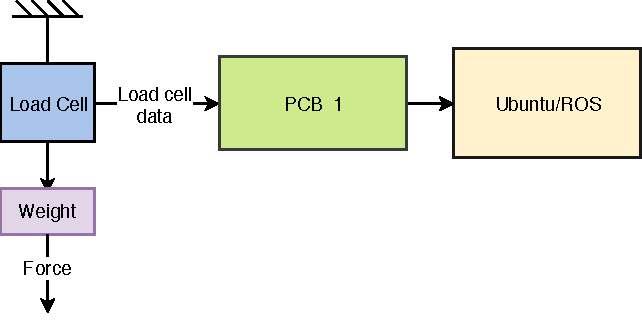
\includegraphics[width=80mm]{fig/methods/Load_Cell_Calibration.pdf}
	\end{center}
	\vspace{-4mm}
	\caption[Block Diagram of the Load Cell Calibration Setup]
	{Block Diagram of the Load Cell Calibration Setup}
	\label{fig:Calib_setup_LC}
	\vspace{-2mm}
\end{figure}

	The calibration equation for the load cell is following:
\begin{equation}
F_{m} = adc_{lc}*a_{lc} + b_{lc}
\end{equation}

	where $adc_{lc}$ is acquired ADC data from the load cell; $a_{lc}$ and $b_{lc}$ are constants of the linear equation.

\begin{figure}[h]
	\begin{center}
	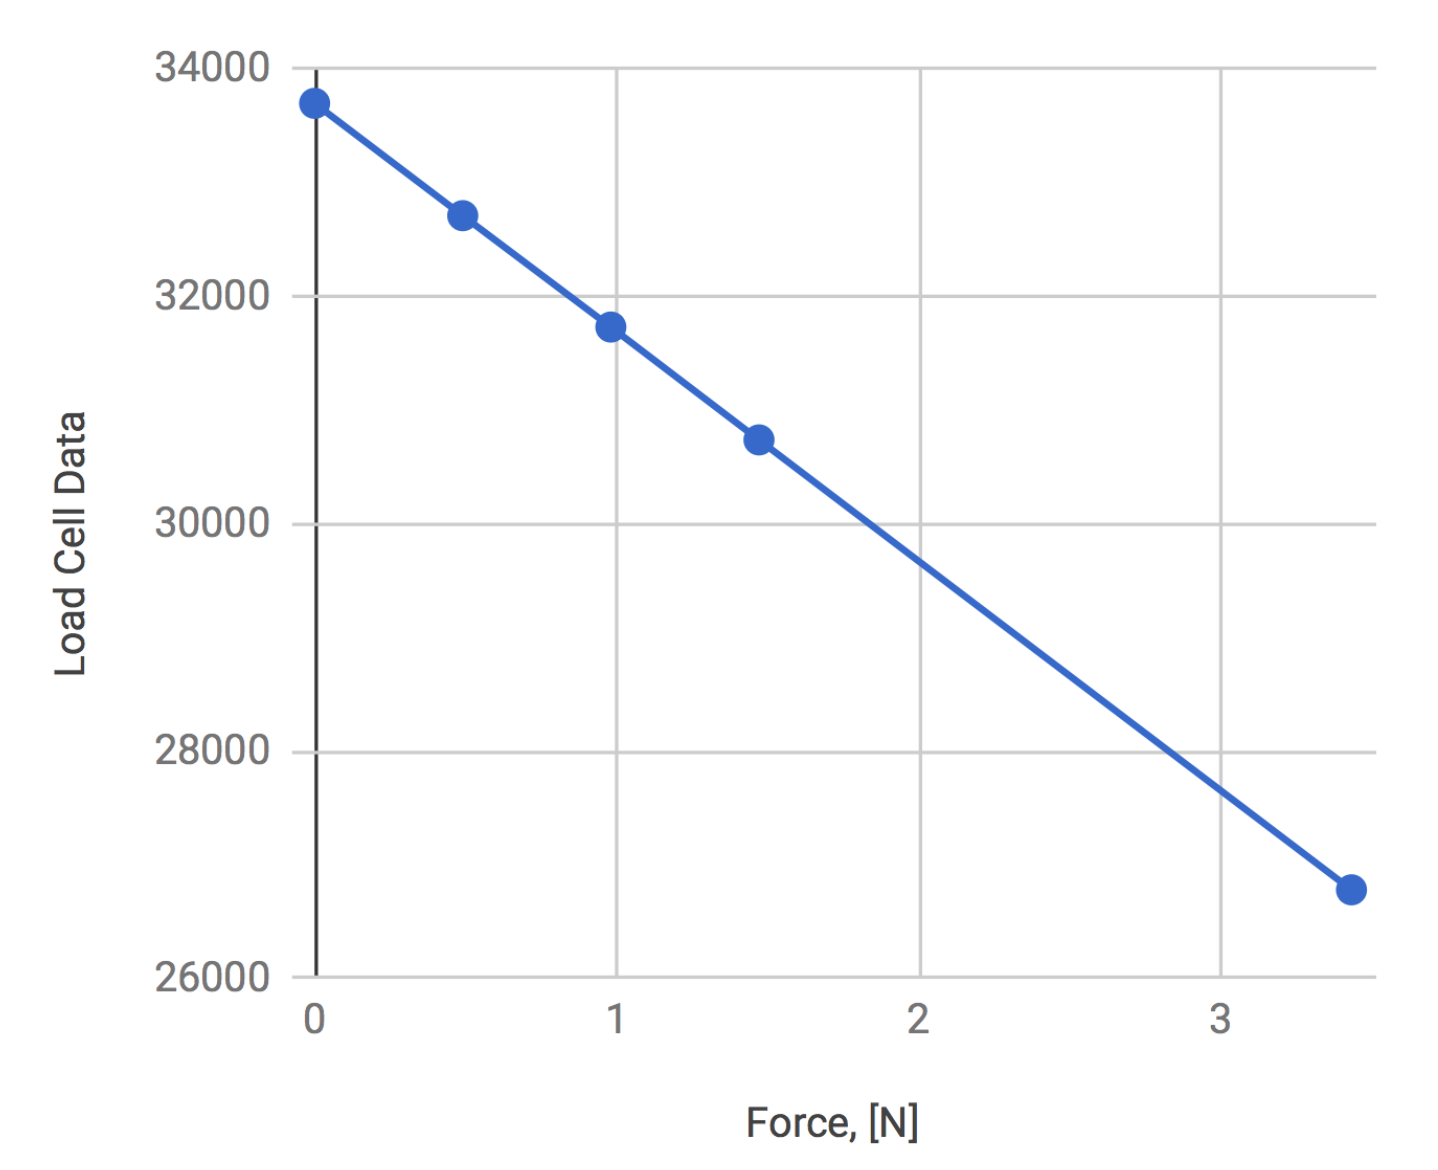
\includegraphics[width=80mm]{fig/methods/load_cell_calib_data.png}
	\end{center}
	\vspace{-4mm}
	\caption[Load Cell Calibration Result]
	{Load Cell Calibration Result}
	\label{fig:LC_calib_res}
	\vspace{-2mm}
\end{figure}

	Calibration resulted in parameters of the linear equation being  $a_{lc} = -4.95 \cdot 10^{-4}$ and $b_{lc} = 16.6$. These values were used to find magnitude of the applied force on the tool end during X-Y and Z devices calibration.

\section{Results}
\label{sec:res}

\subsection{Calibration Results and Sensors Characteristics}
\label{ssec:Cal_Res}

The calibration results are shown on Figures \ref{fig:XY_calib_res}, \ref{fig:Z_calib_res}, where blue dots are sensor readings and the calibration function shown as a red line. The results for the Z device are presented on Figure \ref{fig:Z_calib_sen}. As an alternative method to evaluate forces exerted in a Z-direction we used joint effort readings (Figure \ref{fig:Z_joint_effort}). This method is simple to implement by subscribing to the joint efforts from the daVinci controller and can be used for performance comparison with created Z-device.

The performance of the created devices was evaluated using standard sensor characteristics, such as absolute error, signal to noise ratio, root mean square error, sensitivity, hysteresis, and measurement range.

All the following infromation about sensor chracteristics is from \cite{kalantar-zadeh_sensors_2013}.

\begin{figure}[h]%
\label{fig:XY_calib_res}%
\centering
\subfigure[X-direction]{%
\label{fig:X_calib_res}%
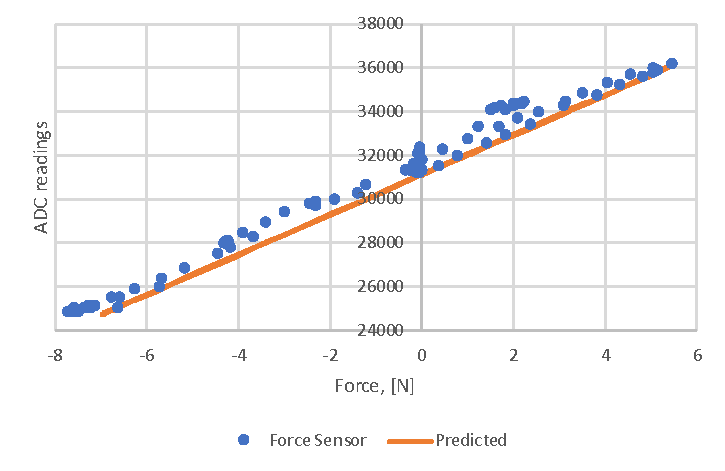
\includegraphics[width=90mm]{fig/results/force_pred_x.pdf}}%
\qquad
\subfigure[Y-direction]{%
\label{fig:Y_calib_res}%
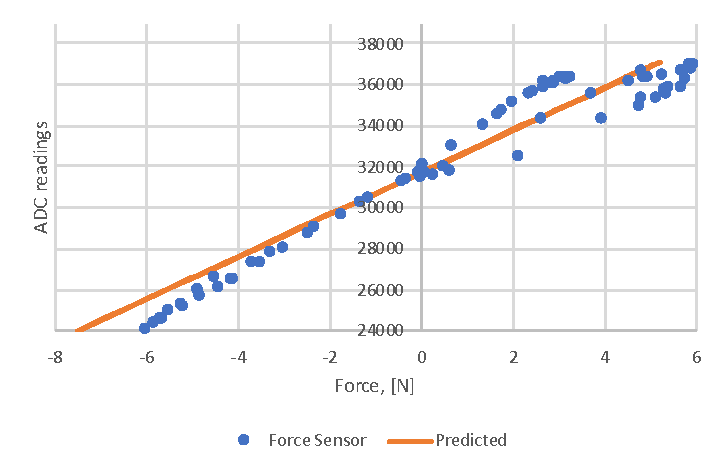
\includegraphics[width=90mm]{fig/results/force_pred_y.pdf}}%
\caption{Calibration Results of XY Device}
\end{figure}

\begin{figure}[h]%
\label{fig:Z_calib_res}%
\centering
\subfigure[Z Device]{%
\label{fig:Z_calib_sen}%
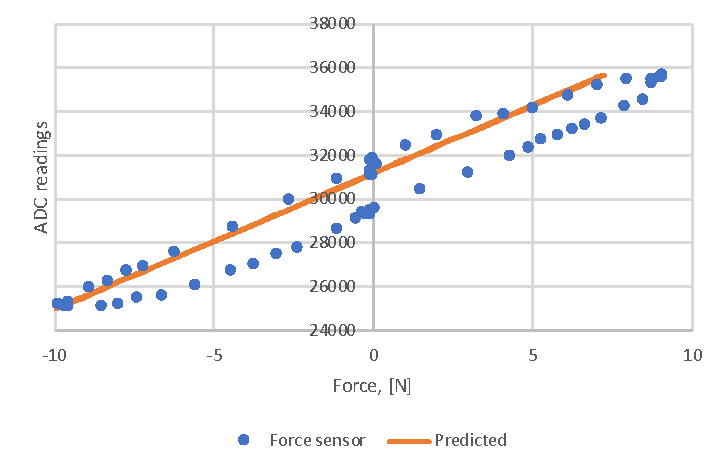
\includegraphics[width=90mm]{fig/results/force_pred_z.pdf}}%
\qquad
\subfigure[Joint Effort]{%
\label{fig:Z_joint_effort}%
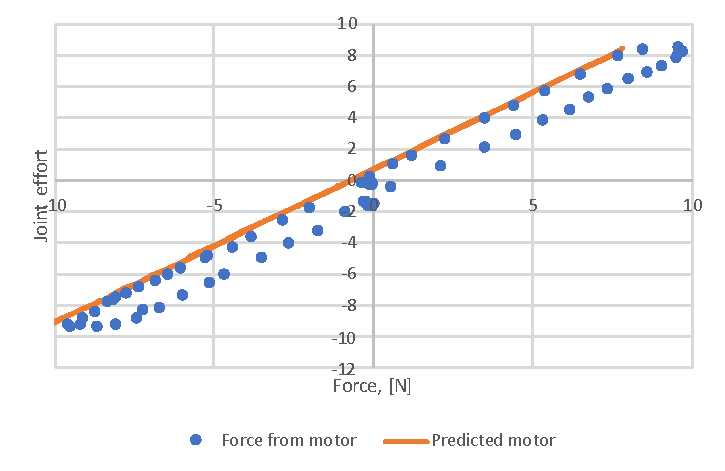
\includegraphics[width=90mm]{fig/results/force_pred_z_effort.pdf}}%
\caption{Calibration Results in Z-direction}
\end{figure}

The accuracy of the developed sensory systems was assessed using the Root Mean Square Error (RMSE), which is:
\begin{equation}
RMSE = \sqrt{\frac{\sum_{i=1}^{n}{{(\hat{y_i} - y_i)}^2}}{n}}
\end{equation}
where $\hat{y_i}$ is predicted with equation (\ref{eq:calib_eq}) force value ; $y_i$ is observed "true" force value found using load cell and Polaris; $n$ is number of observations.

Error is the difference between the actual value of the force and the value produced by the system (Equation \ref{eq:error}). Errors are related to accuracy and can be caused by different sources. 

\begin{equation}\label{eq:error}
error = \hat{y_i} - y_i
\end{equation}

One of the measurements of signal quality is signal-to-noise ratio (SNR). A higher value of SNR means the clear acquisitions with low signal distortions and artifacts caused by unwanted noise. It is defined as:

\begin{equation}
SNR=\frac{\mu}{\sigma}
\end{equation}
where $\mu$ is mean value of signal, $\sigma$ is standard deviation of noise.

The slope of the calibration curve is used for the sensitivity $S$ calculation.

\begin{equation}
S = Dy/Dx
\end{equation}
where $Dy$ is the incremental change in the sensor’s output, $Dx$ is the incremental change of the force. 

Resolution is the smallest change of the applied force that gives a noticeable change in the sensor output, it is limited by the signal noise.

Linearity of the system is proximity of the calibration curve to the straight line. $R^2$ is used to evaluate linearity by measuring closeness of the measured data to the fitted regression line.

Hysteresis is the difference between sensor outputs when the sensor is loaded versus unloaded.

The measurement range consists of the maximum and minimum values of the force that can be measured with created systems. For created system it corresponds to force values, when the output signal reaches saturation. However, for Z-directional measurements, when z-component of the applied force was higher than 12 N it caused sliding of the sterile adapter. Which meaning physical limitation of the system.

Precision represents ability of the system to give the the same output under the same conditions. The precision of the system was assessed by the standard deviation of the sensor outputs, when similar forces were applied. 

All sensor characteristics were calculated for X-Y device, Z-device, and Z-direction evaluation joint effort method and provided in the Table \ref{tab:SenChar}.

\begin{table}[h]
\caption {Sensors Characteristics} \label{tab:SenChar} 
\begin{center}
\begin{tabular}{ | c | c | c | c | c | } 
\hline
 &  X-sensor & Y-sensor & Z-sensor & Joint Effort \\ 
\hline
Error $\pm$ SD, N & $0.059 \pm 0.435$ & $0.017 \pm 0.755$ & $-0.716 \pm 1.324$ & $-1.411 \pm 0.672$ \\ 
\hline
RMSE & 0.44 & 0.75 & 1.5 & 1.56 \\ 
\hline
S/N & 2888 & 3041 & 114 & 566 \\
\hline
Noise SD, N & 0.011 & 0.004 & 0.115 & 0.017 \\
\hline
Sensitivity & 911 & 1030 & 618 & 0.977 \\
\hline
Precision, N & 0.4 & 0.65 & 0.63 & 0.35 \\
\hline
Resolution, N & 0.03 & 0.02 & 0.2 & 0.03 \\
\hline
$R^2$ & 0.965 & 0.924 & 0.938 & 0.963 \\
\hline
Range, N & -19 to 23 & -18 to 20 & -29 to 34 & -12 to 12 \\
\hline
Hysteresis, N & 0.99 & 2.4 & 2.8 & 1.2 \\
\hline
\end{tabular}
\end{center}
\end{table}

\subsection{Calibration Curve Dependence from Sterile Adapter Position}
	\label{sec:DisExp}
	Movement of sterile adapter joint causes change of the length	Position of sterile adapter is acquired from daVinci controller.
	
\begin{figure}[h]%
\label{fig:X_position_dep}%
\centering
\subfigure[Constant a]{%
\label{fig:X_con_a}%
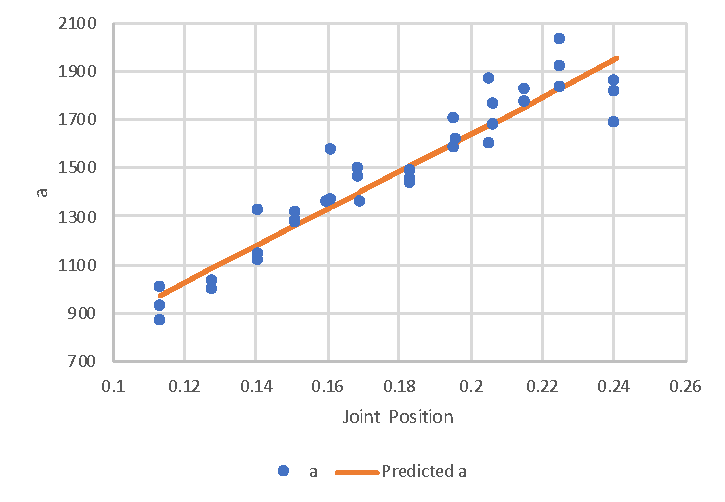
\includegraphics[width=90mm]{fig/results/a_dist_dep_x.pdf}}%
\qquad
\subfigure[Constant b]{%
\label{fig:X_con_b}%
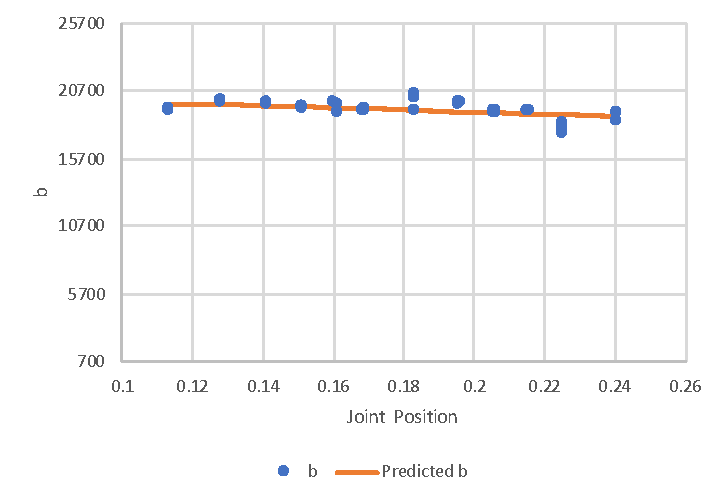
\includegraphics[width=90mm]{fig/results/b_dist_dep_x.pdf}}%
\caption{Sterile Adapter Position Calibration Results for X-direction}
\end{figure}

\begin{figure}[h]%
\label{fig:Y_position_dep}%
\centering
\subfigure[Constant a]{%
\label{fig:Y_con_a}%
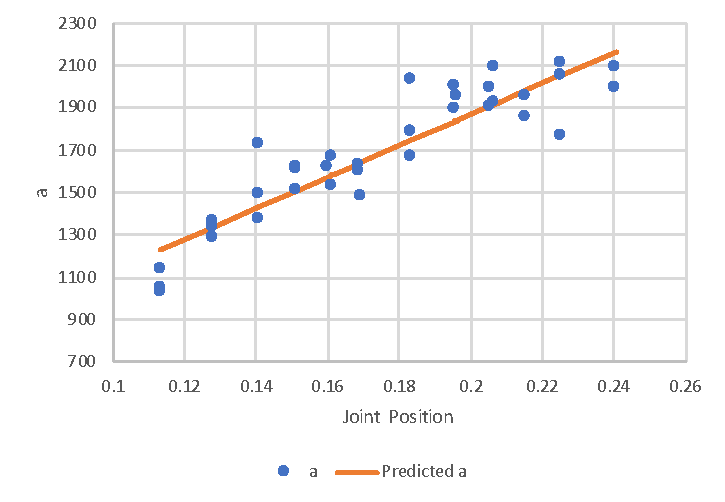
\includegraphics[width=90mm]{fig/results/a_dist_dep_y.pdf}}%
\qquad
\subfigure[Constant b]{%
\label{fig:Y_con_b}%
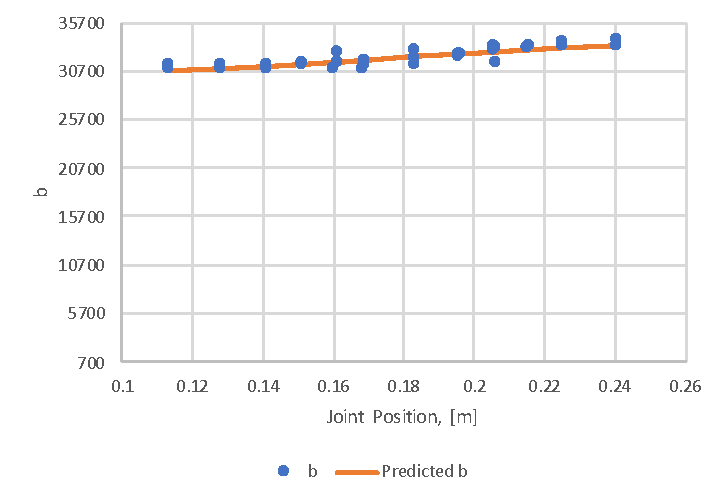
\includegraphics[width=90mm]{fig/results/b_dist_dep_y.pdf}}%
\caption{Sterile Adapter Position Calibration Results for Y-direction}
\end{figure}







